\documentclass[11pt,a4paper]{article}
\usepackage[utf8]{inputenc}
\usepackage[T1]{fontenc}
\usepackage{amsmath,amssymb}
\usepackage{graphicx}
\usepackage{booktabs}
\usepackage{tabularx}
\usepackage{geometry}
\usepackage{float}
\usepackage{xcolor}
\usepackage[hidelinks]{hyperref}
\usepackage{url}\def\UrlBreaks{\do\_\do\/\do\.\do\-}\urlstyle{tt}
\geometry{margin=2.2cm}
\graphicspath{{../results/figures/900d9f88a8_58c9f38705cd/}}
\emergencystretch=2em

% ---------------------------------------------------------------------------------------------
% Number policy. Every \QKD... macro is generated by Optimization/report/make_numbers.py from
% results/MANIFEST.json (results/NUMBERS.md lists the source file of each). Numbers typed directly
% in this file carry a dagger and are copied from the result file named next to them, or from
% STATUS.md, which quotes those files.
% ---------------------------------------------------------------------------------------------
% AUTO-GENERATED by Optimization/report/make_numbers.py from results/MANIFEST.json -- DO NOT EDIT.
% 127 values. Sources: see results/NUMBERS.md.
\providecommand{\QKDLimRefHorizonFour}{}\renewcommand{\QKDLimRefHorizonFour}{130.44}
\providecommand{\QKDLimRefHorizonFive}{}\renewcommand{\QKDLimRefHorizonFive}{160.61}
\providecommand{\QKDLimRefHorizonSix}{}\renewcommand{\QKDLimRefHorizonSix}{172.62}
\providecommand{\QKDLimRefHorizonSeven}{}\renewcommand{\QKDLimRefHorizonSeven}{178.67}
\providecommand{\QKDLimRefHorizonEight}{}\renewcommand{\QKDLimRefHorizonEight}{182.09}
\providecommand{\QKDLimRefHorizonNine}{}\renewcommand{\QKDLimRefHorizonNine}{184.16}
\providecommand{\QKDLimNewColdPctWithin}{}\renewcommand{\QKDLimNewColdPctWithin}{100.0}
\providecommand{\QKDLimNewColdRegretMax}{}\renewcommand{\QKDLimNewColdRegretMax}{\ensuremath{9.06\times 10^{-14}}}
\providecommand{\QKDLimNewColdRegretMedian}{}\renewcommand{\QKDLimNewColdRegretMedian}{\ensuremath{2.37\times 10^{-15}}}
\providecommand{\QKDLimTailNewColdPctWithin}{}\renewcommand{\QKDLimTailNewColdPctWithin}{100.0}
\providecommand{\QKDLimTailNewColdRegretMax}{}\renewcommand{\QKDLimTailNewColdRegretMax}{\ensuremath{6.47\times 10^{-13}}}
\providecommand{\QKDLimNewWarmPctWithin}{}\renewcommand{\QKDLimNewWarmPctWithin}{100.0}
\providecommand{\QKDLimNewWarmRegretMax}{}\renewcommand{\QKDLimNewWarmRegretMax}{\ensuremath{1.03\times 10^{-13}}}
\providecommand{\QKDLimNewWarmRegretMedian}{}\renewcommand{\QKDLimNewWarmRegretMedian}{\ensuremath{3.81\times 10^{-15}}}
\providecommand{\QKDLimTailNewWarmPctWithin}{}\renewcommand{\QKDLimTailNewWarmPctWithin}{100.0}
\providecommand{\QKDLimTailNewWarmRegretMax}{}\renewcommand{\QKDLimTailNewWarmRegretMax}{\ensuremath{9.50\times 10^{-13}}}
\providecommand{\QKDLimLookupPctWithin}{}\renewcommand{\QKDLimLookupPctWithin}{81.6}
\providecommand{\QKDLimLookupRegretMax}{}\renewcommand{\QKDLimLookupRegretMax}{\ensuremath{2.17\times 10^{-2}}}
\providecommand{\QKDLimLookupRegretMedian}{}\renewcommand{\QKDLimLookupRegretMedian}{\ensuremath{1.36\times 10^{-9}}}
\providecommand{\QKDLimTailLookupPctWithin}{}\renewcommand{\QKDLimTailLookupPctWithin}{24.6}
\providecommand{\QKDLimTailLookupRegretMax}{}\renewcommand{\QKDLimTailLookupRegretMax}{\ensuremath{2.31\times 10^{1}}}
\providecommand{\QKDLimXcheckMainPctAgree}{}\renewcommand{\QKDLimXcheckMainPctAgree}{98.1}
\providecommand{\QKDLimXcheckMainWeak}{}\renewcommand{\QKDLimXcheckMainWeak}{0}
\providecommand{\QKDLimXcheckTailPctAgree}{}\renewcommand{\QKDLimXcheckTailPctAgree}{87.8}
\providecommand{\QKDLimXcheckTailWeak}{}\renewcommand{\QKDLimXcheckTailWeak}{0}
\providecommand{\QKDLimSweepMsPerPoint}{}\renewcommand{\QKDLimSweepMsPerPoint}{4.27}
\providecommand{\QKDLimSweepCompileS}{}\renewcommand{\QKDLimSweepCompileS}{80.9}
\providecommand{\QKDLimNewWarmTVFour}{}\renewcommand{\QKDLimNewWarmTVFour}{\ensuremath{2.38\times 10^{-3}}}
\providecommand{\QKDLimNewWarmTVNine}{}\renewcommand{\QKDLimNewWarmTVNine}{\ensuremath{6.54\times 10^{-4}}}
\providecommand{\QKDLimDASecMin}{}\renewcommand{\QKDLimDASecMin}{5.8}
\providecommand{\QKDLimDASecMax}{}\renewcommand{\QKDLimDASecMax}{17.6}
\providecommand{\QKDLimWarmDeviceUs}{}\renewcommand{\QKDLimWarmDeviceUs}{1199}
\providecommand{\QKDLimWarmEndToEndUs}{}\renewcommand{\QKDLimWarmEndToEndUs}{1466}
\providecommand{\QKDLimLookupDeviceUs}{}\renewcommand{\QKDLimLookupDeviceUs}{7.7}
\providecommand{\QKDLimLookupEndToEndUs}{}\renewcommand{\QKDLimLookupEndToEndUs}{10.0}
\providecommand{\QKDLimLiteralRefHorizonFour}{}\renewcommand{\QKDLimLiteralRefHorizonFour}{18.97}
\providecommand{\QKDLimLiteralRefHorizonFive}{}\renewcommand{\QKDLimLiteralRefHorizonFive}{104.53}
\providecommand{\QKDLimLiteralRefHorizonSix}{}\renewcommand{\QKDLimLiteralRefHorizonSix}{129.48}
\providecommand{\QKDLimLiteralRefHorizonSeven}{}\renewcommand{\QKDLimLiteralRefHorizonSeven}{140.00}
\providecommand{\QKDLimLiteralRefHorizonEight}{}\renewcommand{\QKDLimLiteralRefHorizonEight}{145.85}
\providecommand{\QKDLimLiteralRefHorizonNine}{}\renewcommand{\QKDLimLiteralRefHorizonNine}{149.31}
\providecommand{\QKDLimLiteralNewColdPctWithin}{}\renewcommand{\QKDLimLiteralNewColdPctWithin}{100.0}
\providecommand{\QKDLimLiteralNewColdRegretMax}{}\renewcommand{\QKDLimLiteralNewColdRegretMax}{\ensuremath{2.98\times 10^{-14}}}
\providecommand{\QKDLimLiteralNewColdRegretMedian}{}\renewcommand{\QKDLimLiteralNewColdRegretMedian}{\ensuremath{5.93\times 10^{-15}}}
\providecommand{\QKDLimLiteralTailNewColdPctWithin}{}\renewcommand{\QKDLimLiteralTailNewColdPctWithin}{97.9}
\providecommand{\QKDLimLiteralTailNewColdRegretMax}{}\renewcommand{\QKDLimLiteralTailNewColdRegretMax}{\ensuremath{8.74\times 10^{-2}}}
\providecommand{\QKDLimLiteralNewWarmPctWithin}{}\renewcommand{\QKDLimLiteralNewWarmPctWithin}{100.0}
\providecommand{\QKDLimLiteralNewWarmRegretMax}{}\renewcommand{\QKDLimLiteralNewWarmRegretMax}{\ensuremath{6.65\times 10^{-14}}}
\providecommand{\QKDLimLiteralNewWarmRegretMedian}{}\renewcommand{\QKDLimLiteralNewWarmRegretMedian}{\ensuremath{1.39\times 10^{-14}}}
\providecommand{\QKDLimLiteralTailNewWarmPctWithin}{}\renewcommand{\QKDLimLiteralTailNewWarmPctWithin}{98.6}
\providecommand{\QKDLimLiteralTailNewWarmRegretMax}{}\renewcommand{\QKDLimLiteralTailNewWarmRegretMax}{\ensuremath{5.27\times 10^{-2}}}
\providecommand{\QKDLimLiteralLookupPctWithin}{}\renewcommand{\QKDLimLiteralLookupPctWithin}{76.5}
\providecommand{\QKDLimLiteralLookupRegretMax}{}\renewcommand{\QKDLimLiteralLookupRegretMax}{\ensuremath{4.19\times 10^{-4}}}
\providecommand{\QKDLimLiteralLookupRegretMedian}{}\renewcommand{\QKDLimLiteralLookupRegretMedian}{\ensuremath{1.72\times 10^{-8}}}
\providecommand{\QKDLimLiteralTailLookupPctWithin}{}\renewcommand{\QKDLimLiteralTailLookupPctWithin}{24.0}
\providecommand{\QKDLimLiteralTailLookupRegretMax}{}\renewcommand{\QKDLimLiteralTailLookupRegretMax}{\ensuremath{2.62\times 10^{-1}}}
\providecommand{\QKDLimLiteralSweepMsPerPoint}{}\renewcommand{\QKDLimLiteralSweepMsPerPoint}{5.35}
\providecommand{\QKDLimLiteralSweepCompileS}{}\renewcommand{\QKDLimLiteralSweepCompileS}{82.0}
\providecommand{\QKDLimLiteralNewWarmTVFour}{}\renewcommand{\QKDLimLiteralNewWarmTVFour}{\ensuremath{9.63\times 10^{-3}}}
\providecommand{\QKDLimLiteralNewWarmTVNine}{}\renewcommand{\QKDLimLiteralNewWarmTVNine}{\ensuremath{2.72\times 10^{-3}}}
\providecommand{\QKDLegacyRefHorizonFour}{}\renewcommand{\QKDLegacyRefHorizonFour}{148.17}
\providecommand{\QKDLegacyRefHorizonFive}{}\renewcommand{\QKDLegacyRefHorizonFive}{171.43}
\providecommand{\QKDLegacyRefHorizonSix}{}\renewcommand{\QKDLegacyRefHorizonSix}{180.97}
\providecommand{\QKDLegacyRefHorizonSeven}{}\renewcommand{\QKDLegacyRefHorizonSeven}{185.97}
\providecommand{\QKDLegacyRefHorizonEight}{}\renewcommand{\QKDLegacyRefHorizonEight}{188.87}
\providecommand{\QKDLegacyRefHorizonNine}{}\renewcommand{\QKDLegacyRefHorizonNine}{190.67}
\providecommand{\QKDLegacyNewColdPctWithin}{}\renewcommand{\QKDLegacyNewColdPctWithin}{100.0}
\providecommand{\QKDLegacyNewColdRegretMax}{}\renewcommand{\QKDLegacyNewColdRegretMax}{\ensuremath{7.62\times 10^{-9}}}
\providecommand{\QKDLegacyNewColdRegretMedian}{}\renewcommand{\QKDLegacyNewColdRegretMedian}{\ensuremath{6.93\times 10^{-14}}}
\providecommand{\QKDLegacyTailNewColdPctWithin}{}\renewcommand{\QKDLegacyTailNewColdPctWithin}{99.3}
\providecommand{\QKDLegacyTailNewColdRegretMax}{}\renewcommand{\QKDLegacyTailNewColdRegretMax}{\ensuremath{1.14\times 10^{-1}}}
\providecommand{\QKDLegacyNewWarmPctWithin}{}\renewcommand{\QKDLegacyNewWarmPctWithin}{100.0}
\providecommand{\QKDLegacyNewWarmRegretMax}{}\renewcommand{\QKDLegacyNewWarmRegretMax}{\ensuremath{1.40\times 10^{-9}}}
\providecommand{\QKDLegacyNewWarmRegretMedian}{}\renewcommand{\QKDLegacyNewWarmRegretMedian}{\ensuremath{5.87\times 10^{-13}}}
\providecommand{\QKDLegacyTailNewWarmPctWithin}{}\renewcommand{\QKDLegacyTailNewWarmPctWithin}{100.0}
\providecommand{\QKDLegacyTailNewWarmRegretMax}{}\renewcommand{\QKDLegacyTailNewWarmRegretMax}{\ensuremath{2.61\times 10^{-9}}}
\providecommand{\QKDLegacyLookupPctWithin}{}\renewcommand{\QKDLegacyLookupPctWithin}{81.7}
\providecommand{\QKDLegacyLookupRegretMax}{}\renewcommand{\QKDLegacyLookupRegretMax}{\ensuremath{3.79\times 10^{-1}}}
\providecommand{\QKDLegacyLookupRegretMedian}{}\renewcommand{\QKDLegacyLookupRegretMedian}{\ensuremath{1.37\times 10^{-9}}}
\providecommand{\QKDLegacyTailLookupPctWithin}{}\renewcommand{\QKDLegacyTailLookupPctWithin}{24.6}
\providecommand{\QKDLegacyTailLookupRegretMax}{}\renewcommand{\QKDLegacyTailLookupRegretMax}{\ensuremath{5.46\times 10^{-1}}}
\providecommand{\QKDLegacyOldDAPctWithin}{}\renewcommand{\QKDLegacyOldDAPctWithin}{3.7}
\providecommand{\QKDLegacyOldDARegretMax}{}\renewcommand{\QKDLegacyOldDARegretMax}{\ensuremath{1.26\times 10^{0}}}
\providecommand{\QKDLegacyOldDARegretMedian}{}\renewcommand{\QKDLegacyOldDARegretMedian}{\ensuremath{1.42\times 10^{-2}}}
\providecommand{\QKDLegacyTailOldDAPctWithin}{}\renewcommand{\QKDLegacyTailOldDAPctWithin}{0.0}
\providecommand{\QKDLegacyTailOldDARegretMax}{}\renewcommand{\QKDLegacyTailOldDARegretMax}{\ensuremath{8.91\times 10^{-1}}}
\providecommand{\QKDLegacyOldHessianPctWithin}{}\renewcommand{\QKDLegacyOldHessianPctWithin}{96.3}
\providecommand{\QKDLegacyOldHessianRegretMax}{}\renewcommand{\QKDLegacyOldHessianRegretMax}{\ensuremath{2.68\times 10^{1}}}
\providecommand{\QKDLegacyOldHessianRegretMedian}{}\renewcommand{\QKDLegacyOldHessianRegretMedian}{\ensuremath{1.14\times 10^{-11}}}
\providecommand{\QKDLegacyTailOldHessianPctWithin}{}\renewcommand{\QKDLegacyTailOldHessianPctWithin}{95.8}
\providecommand{\QKDLegacyTailOldHessianRegretMax}{}\renewcommand{\QKDLegacyTailOldHessianRegretMax}{\ensuremath{4.67\times 10^{-1}}}
\providecommand{\QKDLegacyOldFoRPctWithin}{}\renewcommand{\QKDLegacyOldFoRPctWithin}{81.7}
\providecommand{\QKDLegacyOldFoRRegretMax}{}\renewcommand{\QKDLegacyOldFoRRegretMax}{\ensuremath{9.65\times 10^{1}}}
\providecommand{\QKDLegacyOldFoRRegretMedian}{}\renewcommand{\QKDLegacyOldFoRRegretMedian}{\ensuremath{2.03\times 10^{-11}}}
\providecommand{\QKDLegacyTailOldFoRPctWithin}{}\renewcommand{\QKDLegacyTailOldFoRPctWithin}{0.0}
\providecommand{\QKDLegacyTailOldFoRRegretMax}{}\renewcommand{\QKDLegacyTailOldFoRRegretMax}{\ensuremath{3.64\times 10^{1}}}
\providecommand{\QKDLegacyXcheckMainPctAgree}{}\renewcommand{\QKDLegacyXcheckMainPctAgree}{97.3}
\providecommand{\QKDLegacyXcheckMainWeak}{}\renewcommand{\QKDLegacyXcheckMainWeak}{0}
\providecommand{\QKDLegacySweepMsPerPoint}{}\renewcommand{\QKDLegacySweepMsPerPoint}{0.63}
\providecommand{\QKDLegacySweepCompileS}{}\renewcommand{\QKDLegacySweepCompileS}{28.1}
\providecommand{\QKDLegacyNewWarmTVFour}{}\renewcommand{\QKDLegacyNewWarmTVFour}{\ensuremath{1.85\times 10^{-3}}}
\providecommand{\QKDLegacyOldDATVFour}{}\renewcommand{\QKDLegacyOldDATVFour}{\ensuremath{7.95\times 10^{-3}}}
\providecommand{\QKDLegacyOldFoRTVFour}{}\renewcommand{\QKDLegacyOldFoRTVFour}{\ensuremath{1.84\times 10^{-3}}}
\providecommand{\QKDLegacyNewWarmTVNine}{}\renewcommand{\QKDLegacyNewWarmTVNine}{\ensuremath{1.86\times 10^{-3}}}
\providecommand{\QKDLegacyOldDATVNine}{}\renewcommand{\QKDLegacyOldDATVNine}{\ensuremath{2.61\times 10^{-3}}}
\providecommand{\QKDLegacyOldFoRTVNine}{}\renewcommand{\QKDLegacyOldFoRTVNine}{\ensuremath{1.85\times 10^{-3}}}
\providecommand{\QKDLimTargetROne}{}\renewcommand{\QKDLimTargetROne}{\ensuremath{9.203\times 10^{-3}}}
\providecommand{\QKDLimTargetRatio}{}\renewcommand{\QKDLimTargetRatio}{1.791}
\providecommand{\QKDLimTargetHorizon}{}\renewcommand{\QKDLimTargetHorizon}{130.4}
\providecommand{\QKDLimTargetCrossing}{}\renewcommand{\QKDLimTargetCrossing}{118.8}
\providecommand{\QKDLimTargetROneDevPct}{}\renewcommand{\QKDLimTargetROneDevPct}{-8\%}
\providecommand{\QKDLimTargetRatioDevPct}{}\renewcommand{\QKDLimTargetRatioDevPct}{+2\%}
\providecommand{\QKDLimTargetHorizonDevPct}{}\renewcommand{\QKDLimTargetHorizonDevPct}{-3\%}
\providecommand{\QKDLimLiteralTargetROne}{}\renewcommand{\QKDLimLiteralTargetROne}{\ensuremath{1.250\times 10^{-3}}}
\providecommand{\QKDLimLiteralTargetRatio}{}\renewcommand{\QKDLimLiteralTargetRatio}{2.734}
\providecommand{\QKDLimLiteralTargetHorizon}{}\renewcommand{\QKDLimLiteralTargetHorizon}{19.0}
\providecommand{\QKDLimLiteralTargetCrossing}{}\renewcommand{\QKDLimLiteralTargetCrossing}{--}
\providecommand{\QKDLimLiteralTargetROneDevPct}{}\renewcommand{\QKDLimLiteralTargetROneDevPct}{-87\%}
\providecommand{\QKDLimLiteralTargetRatioDevPct}{}\renewcommand{\QKDLimLiteralTargetRatioDevPct}{+56\%}
\providecommand{\QKDLimLiteralTargetHorizonDevPct}{}\renewcommand{\QKDLimLiteralTargetHorizonDevPct}{-86\%}
\providecommand{\QKDLegacyTargetROne}{}\renewcommand{\QKDLegacyTargetROne}{\ensuremath{1.090\times 10^{-2}}}
\providecommand{\QKDLegacyTargetRatio}{}\renewcommand{\QKDLegacyTargetRatio}{1.790}
\providecommand{\QKDLegacyTargetHorizon}{}\renewcommand{\QKDLegacyTargetHorizon}{148.2}
\providecommand{\QKDLegacyTargetCrossing}{}\renewcommand{\QKDLegacyTargetCrossing}{134.1}
\providecommand{\QKDLegacyTargetROneDevPct}{}\renewcommand{\QKDLegacyTargetROneDevPct}{+9\%}
\providecommand{\QKDLegacyTargetRatioDevPct}{}\renewcommand{\QKDLegacyTargetRatioDevPct}{+2\%}
\providecommand{\QKDLegacyTargetHorizonDevPct}{}\renewcommand{\QKDLegacyTargetHorizonDevPct}{+10\%}

\newcommand{\typed}{\textsuperscript{\dag}}
\newcommand{\plim}{\texttt{lim}}
\newcommand{\limlit}{\texttt{lim\_literal}}
\newcommand{\legacy}{\texttt{legacy}}
\newcommand{\esec}{\varepsilon_{\mathrm{sec}}}
\newcommand{\ecor}{\varepsilon_{\mathrm{cor}}}
\newcommand{\fitbox}[1]{\resizebox{\ifdim\width>\linewidth\linewidth\else\width\fi}{!}{#1}}

\title{Optimal Parameters for Finite-Key Decoy-State BB84\\
under the Lim et al.\ (2014) Bounds:\\
a Verified Optimizer, a Corrected Model, and a Benchmark Protocol for Surrogates\\[6pt]
\large Final report of the \texttt{optimizer-jax-rework} branch (supersedes all earlier reports)}
\author{Shek Lun Leung}
\date{November 2026}

\begin{document}
\maketitle

\begin{abstract}
We compute the parameters that maximise the secret key rate $R$ of finite-key decoy-state BB84 under the security
bounds of Lim, Curty, Walenta, Xu and Zbinden (PRA 89, 022307, 2014): signal and decoy intensities, their
probabilities and the basis probability, as functions of fiber length $L\in[0,200]$\,km and block size
$n_X\in[10^4,10^9]$.

An audit of the earlier pipeline found four problems:
\begin{itemize}
\item the earlier key-rate code used the $X$-basis detection count where Eq.~(4) of the paper requires the
  $Z$-basis error count;
\item it departed from the paper in four further model settings;
\item the optimizers that produced the neural-network training labels did not reach the optimum;
\item most headline numbers of the earlier reports could not be reproduced.
\end{itemize}

We present a corrected model and a JAX optimizer whose output is verified against an independently built
reference:
\begin{itemize}
\item The corrected model agrees with an independent re-implementation to $\le2\times10^{-13}$ in $\ell$ and
  reproduces the paper's three stated numbers to within 8\,\%.
\item The optimizer uses an exact Hessian, penalty-free constraints and continuation in $L$. Its relative regret
  is at most \QKDLimNewWarmRegretMax\ on the bulk grid and \QKDLimTailNewWarmRegretMax\ on a dense grid near the
  maximal distance, at 100\,\% of scored points.
\item For comparison, the earlier dual-annealing run is within $10^{-6}$ at \QKDLegacyOldDAPctWithin\,\% of
  points, and the run that produced the neural-network labels at \QKDLegacyOldFoRPctWithin\,\% (bulk) and
  \QKDLegacyTailOldFoRPctWithin\,\% (tail).
\item The optimal parameters vary smoothly with $L$, apart from two switches between competing local optima
  ($n_X=10^5$ near 130.5\,km, $n_X=10^6$ near 118.5\,km). The optimizer detects and logs both.
\item A warm-started single-point solve takes \QKDLimWarmDeviceUs\,$\mu$s on a laptop CPU.
\end{itemize}

All earlier neural-network results are withdrawn. We specify, in advance, the protocol by which a retrained
classical network and a quantum machine-learning model will be benchmarked against this reference.
\end{abstract}

\tableofcontents
\newpage

%======================================================================
\section{Introduction and scope}
%======================================================================
Decoy-state BB84 with finite-key security needs five free parameters per operating point:
\[
  p = (\mu_1,\mu_2,P_{\mu_1},P_{\mu_2},q_x),\qquad \mu_3 = 2\times10^{-4}\ \text{fixed},\qquad P_{\mu_3}=1-P_{\mu_1}-P_{\mu_2}.
\]
The optimal $p$ depends on the channel (fiber length $L$) and on the block size $n_X$. Re-optimising whenever the
channel changes is the motivation for fast surrogates: neural networks, and next, quantum machine learning (QML).

A surrogate can be no better than (a) the physics model that defines $R$ and (b) the optimizer that produces its
training labels. This report establishes both, and the yardstick against which a surrogate is scored.

\paragraph{Document history.} This report supersedes three earlier documents (Appendix~\ref{app:supersede}):
\begin{itemize}
\item the MSc thesis report, May 2025 (\path{Project_Report/...Final_Report.pdf});
\item the results report, January/March 2026 (\path{result_report/results_report.tex});
\item the interview slides derived from that report.
\end{itemize}
Numbers in those documents should not be cited. Where they conflict with this report, this report holds.

\paragraph{Contributions.}
\begin{enumerate}
\item A physics model (preset \plim) that is audited against the paper equation by equation. It documents every
  choice the paper leaves open and is validated against an independent implementation (Section~\ref{sec:model}).
\item A penalty-free JAX optimizer with exact second-order steps and per-point certificates
  (Section~\ref{sec:optimizer}).
\item A trusted reference and an evaluation protocol. The protocol defines regret, distance horizon, smoothness
  and timing, and requires independent cross-checks (Sections~\ref{sec:protocol}--\ref{sec:results}).
\item A protocol, fixed in advance, for benchmarking surrogate models, including QML (Section~\ref{sec:qml}).
\end{enumerate}

%======================================================================
\section{Model: finite-key decoy-state BB84 (Lim et al.\ 2014)}\label{sec:model}
%======================================================================
\subsection{Channel, detection and error model}
With attenuation $\alpha$, $\eta_{\mathrm{ch}}=10^{-\alpha L/10}$ and $\eta_{\mathrm{sys}}=\eta_{\mathrm{Bob}}\,\eta_{\mathrm{ch}}$.
For intensity $k\in\{\mu_1,\mu_2,\mu_3\}$ with probability $p_k$:
\begin{align}
  D_k &= 1-(1-2p_{\mathrm{dc}})\,e^{-\eta_{\mathrm{sys}}k}, & R_k &= D_k(1+p_{\mathrm{ap}}),\\
  e_k &= p_{\mathrm{dc}} + e_{\mathrm{mis}}\bigl(1-e^{-\eta_{\mathrm{sys}}k}\bigr) + \tfrac{p_{\mathrm{ap}}}{2}D_k .
\end{align}
Both $1-e^{-x}$ terms are evaluated as $-\mathrm{expm1}(-x)$ (Section~\ref{sec:numerics}).

Expected counts are used as the observed counts (no sampling):
\begin{gather}
  N = \frac{n_X}{q_x^2\sum_k p_k R_k},\qquad
  n_{X,k}=Nq_x^2p_kR_k,\quad n_{Z,k}=N(1-q_x)^2p_kR_k,\\
  m_{X,k}=Nq_x^2p_ke_k,\quad m_{Z,k}=N(1-q_x)^2p_ke_k,\qquad
  e_{\mathrm{obs}}=\textstyle\sum_k m_{X,k}/n_X .
\end{gather}

\subsection{Key length (Eqs.~(1)--(5) of the paper)}
Let $\delta(n,\varepsilon)=\sqrt{\tfrac n2\ln\tfrac{21}{\varepsilon}}$ and
$n^\pm_{X,k}=\tfrac{e^{k}}{p_k}\bigl(n_{X,k}\pm\delta(n_X,\esec)\bigr)$. Define $n^\pm_{Z,k}$ likewise with $n_Z$,
and $m^\pm_{Z,k}$ with $m_Z=\sum_k m_{Z,k}$. Let $\tau_j=\sum_k p_k e^{-k}k^j/j!$. Then
\begin{align}
  s_{X,0} &\ge \tau_0\,\frac{\mu_2 n^-_{X,\mu_3}-\mu_3 n^+_{X,\mu_2}}{\mu_2-\mu_3},\\
  s_{X,1} &\ge \frac{\tau_1\mu_1\bigl[n^-_{X,\mu_2}-n^+_{X,\mu_3}-\frac{\mu_2^2-\mu_3^2}{\mu_1^2}\bigl(n^+_{X,\mu_1}-\frac{s_{X,0}}{\tau_0}\bigr)\bigr]}{\mu_1(\mu_2-\mu_3)-\mu_2^2+\mu_3^2},\\
  v_{Z,1} &\le \tau_1\,\frac{m^+_{Z,\mu_2}-m^-_{Z,\mu_3}}{\mu_2-\mu_3},\qquad
  \phi_X \le \frac{v_{Z,1}}{s_{Z,1}}+\gamma\Bigl(\esec,\frac{v_{Z,1}}{s_{Z,1}},s_{Z,1},s_{X,1}\Bigr),\\
  \gamma(a,b,c,d) &= \sqrt{\frac{(c+d)(1-b)b}{cd\ln 2}\,\log_2\!\Bigl(\frac{c+d}{cd(1-b)b}\,\frac{21^2}{a^2}\Bigr)},\\
  \ell &= s_{X,0}+s_{X,1}\bigl(1-h(\phi_X)\bigr)-n_Xf_{\mathrm{EC}}h(e_{\mathrm{obs}})-6\log_2\frac{21}{\esec}-\log_2\frac{2}{\ecor},
  \qquad R=\ell/N .
\end{align}
Here $h$ is the binary entropy. The secrecy parameter is tied to the key length, $\esec=\kappa\ell$ with
$\kappa=10^{-15}$. We take the greatest self-consistent fixed point of $\esec=\kappa\max(\ell(\esec),1)$, found by
monotone iteration and log-bisection, and differentiate it exactly through the implicit-function theorem
(\texttt{custom\_jvp}).

\subsection{Constants and presets}
\begin{table}[H]\centering\small
\begin{tabular}{lll}\toprule
Constant & value (\plim) & note\\\midrule
$\alpha$, $\eta_{\mathrm{Bob}}$, $p_{\mathrm{dc}}$ & 0.2 dB/km, 0.1, $6\times10^{-7}$ & as in the paper\\
$e_{\mathrm{mis}}$, $p_{\mathrm{ap}}$ & $5\times10^{-3}$, $4\times10^{-2}$ & as in the paper\\
$f_{\mathrm{EC}}$, $\ecor$, $\kappa$ & 1.16, $10^{-15}$, $10^{-15}$ & as in the paper\\
$\mu_3$ & $2\times10^{-4}$ & fixed\\
box & $\mu_1<0.9$, $\mu_2<0.5$ & not stated in the paper; same box as all earlier runs\\\bottomrule
\end{tabular}
\caption{Constants of the default preset \plim\ (\texttt{src/qkd\_opt/presets.py}).}
\end{table}

Three presets are used:
\begin{description}
\item[\plim\ (default)] Everything above. The misalignment term uses $\eta_{\mathrm{sys}}$, whereas the paper
  prints $\eta_{\mathrm{ch}}$.
\item[\limlit\ (diagnostic)] The printed $\eta_{\mathrm{ch}}$ in $e_k$.
\item[\legacy] The physics of the earlier code \texttt{src/qkd}: $e_{\mathrm{mis}}=0.01$, $p_{\mathrm{ap}}=0$,
  $\esec=10^{-10}$ fixed, $m_Z=\sum_k n_{X,k}$ (a defect), $R_k=D_k$, and $n^-,m^-$ clamped at 0. It is
  reproduced to $<10^{-8}$ relative in $\ell$ and is used \emph{only} to score the stored earlier runs on the
  objective they were optimised for.
\end{description}

\subsection{Choices the paper leaves open}\label{sec:choices}
The paper does not print the following; each is our stated choice (full list in \texttt{PHYSICS\_DIFF.md}):
\begin{itemize}
\item the expected-count model above;
\item $e_{\mathrm{obs}}$ as the detection-weighted $X$-basis error rate;
\item $\eta_{\mathrm{sys}}$ in the misalignment term;
\item the greatest fixed point for $\esec=\kappa\ell$;
\item dropping the floor in Eq.~(1), a continuous relaxation needed for gradients;
\item clamping $s_{\cdot,0}\ge0$ and dropping the single-photon term when $s_{\cdot,1}\le0$;
\item capping $\phi_X\le\tfrac12$, and setting $\phi_X=\tfrac12$ when $v_{Z,1}/s_{Z,1}\le0$;
\item not clamping $n^-$, $m^-$;
\item the factors $q_x^2$ and $(1-q_x)^2$ for basis sifting;
\item the optimisation box.
\end{itemize}

%----------------------------------------------------------------------
\subsection{Agreement with the paper}\label{sec:targets}
The paper states three numbers. No numerical constant was tuned to them. The one structural choice, $\eta_{\mathrm{sys}}$
versus the printed $\eta_{\mathrm{ch}}$, was made by comparing against these same numbers, so they do not
independently validate that choice.
\begin{table}[H]\centering\small
\fitbox{\begin{tabular}{lccc}\toprule
Preset & $R(0,10^9)$ [paper $\sim10^{-2}$] & $R(100,10^9)/R(100,10^7)$ [$\sim1.75$] & horizon $n_X=10^4$ [$\sim135$\,km]\\\midrule
\plim   & \QKDLimTargetROne\ (\QKDLimTargetROneDevPct) & \QKDLimTargetRatio\ (\QKDLimTargetRatioDevPct) & \QKDLimTargetHorizon\ (\QKDLimTargetHorizonDevPct)\\
\limlit & \QKDLimLiteralTargetROne\ (\QKDLimLiteralTargetROneDevPct) & \QKDLimLiteralTargetRatio\ (\QKDLimLiteralTargetRatioDevPct) & \QKDLimLiteralTargetHorizon\ (\QKDLimLiteralTargetHorizonDevPct)\\
\legacy & \QKDLegacyTargetROne\ (\QKDLegacyTargetROneDevPct) & \QKDLegacyTargetRatio\ (\QKDLegacyTargetRatioDevPct) & \QKDLegacyTargetHorizon\ (\QKDLegacyTargetHorizonDevPct)\\\bottomrule
\end{tabular}}
\caption{Paper targets, with the relative deviation in brackets. The paper's values are read from its text and
Fig.~1, so they are approximate ($\sim$). \plim\ is within 8\,\%. The printed $\eta_{\mathrm{ch}}$ misses all three
by far, so we treat it as a probable typo. This is an inference; the authors have not confirmed it. \legacy\ lands
close only because its errors partly cancel (Table~\ref{tab:chain}).}\label{tab:targets}
\end{table}

\subsection{Effect of each correction}
Table~\ref{tab:chain} applies the corrections from \legacy\ to \plim\ one at a time and re-optimises at each
stage (\path{Optimization/analysis/physics_diff.py}; values\typed\ from
\path{results/physics_diff_a419cc7422_dba94a5ecdc3/}).

\begin{table}[H]\centering\small
\fitbox{\begin{tabular}{llcccc}\toprule
& stage (cumulative) & $R(100,10^4)$ & $R(100,10^9)$ & horizon $10^4$ & horizon $10^9$\\\midrule
0 & \legacy & $2.60\times10^{-6}$ & $9.88\times10^{-5}$ & 148.17 & 190.67\\
1 & expm1 evaluation (numerics only) & $2.60\times10^{-6}$ & $9.88\times10^{-5}$ & 148.17 & 190.67\\
2 & $m_Z$ = $Z$-basis errors (defect fixed) & $5.39\times10^{-6}$ & $1.42\times10^{-4}$ & 148.17 & 190.67\\
3 & $e_{\mathrm{mis}}$ $0.01\to5\times10^{-3}$ & $8.20\times10^{-6}$ & $1.74\times10^{-4}$ & 152.50 & 192.71\\
4 & $p_{\mathrm{ap}}$ $0\to0.04$ in $e_k$ & $1.22\times10^{-6}$ & $7.89\times10^{-5}$ & 133.61 & 182.43\\
5 & $R_k=D_k(1+p_{\mathrm{ap}})$ & $1.47\times10^{-6}$ & $8.57\times10^{-5}$ & 135.37 & 184.17\\
6 & $\esec=\kappa\ell$ & $1.07\times10^{-6}$ & $8.80\times10^{-5}$ & 130.44 & 184.16\\
7 & $n^-,m^-$ not clamped $=$ \plim & $9.91\times10^{-7}$ & $8.54\times10^{-5}$ & 130.44 & 184.16\\
8 & printed $\eta_{\mathrm{ch}}$ $=$ \limlit & $\le0$ & $7.94\times10^{-6}$ & 18.97 & 149.31\\\bottomrule
\end{tabular}}
\caption{Cumulative ablation; $R$ in bits/pulse, horizons in km.
\textbf{Reading:}
(i) Fixing the $m_Z$ defect alone roughly doubles $R$ at $n_X=10^4$.
(ii) Afterpulsing (stages 4--5) shortens the $n_X=10^4$ reach by 17\,km.
(iii) Overall, the earlier physics overstated the $n_X=10^4$ reach by 17.7\,km relative to \plim.}\label{tab:chain}
\end{table}

\begin{figure}[H]\centering
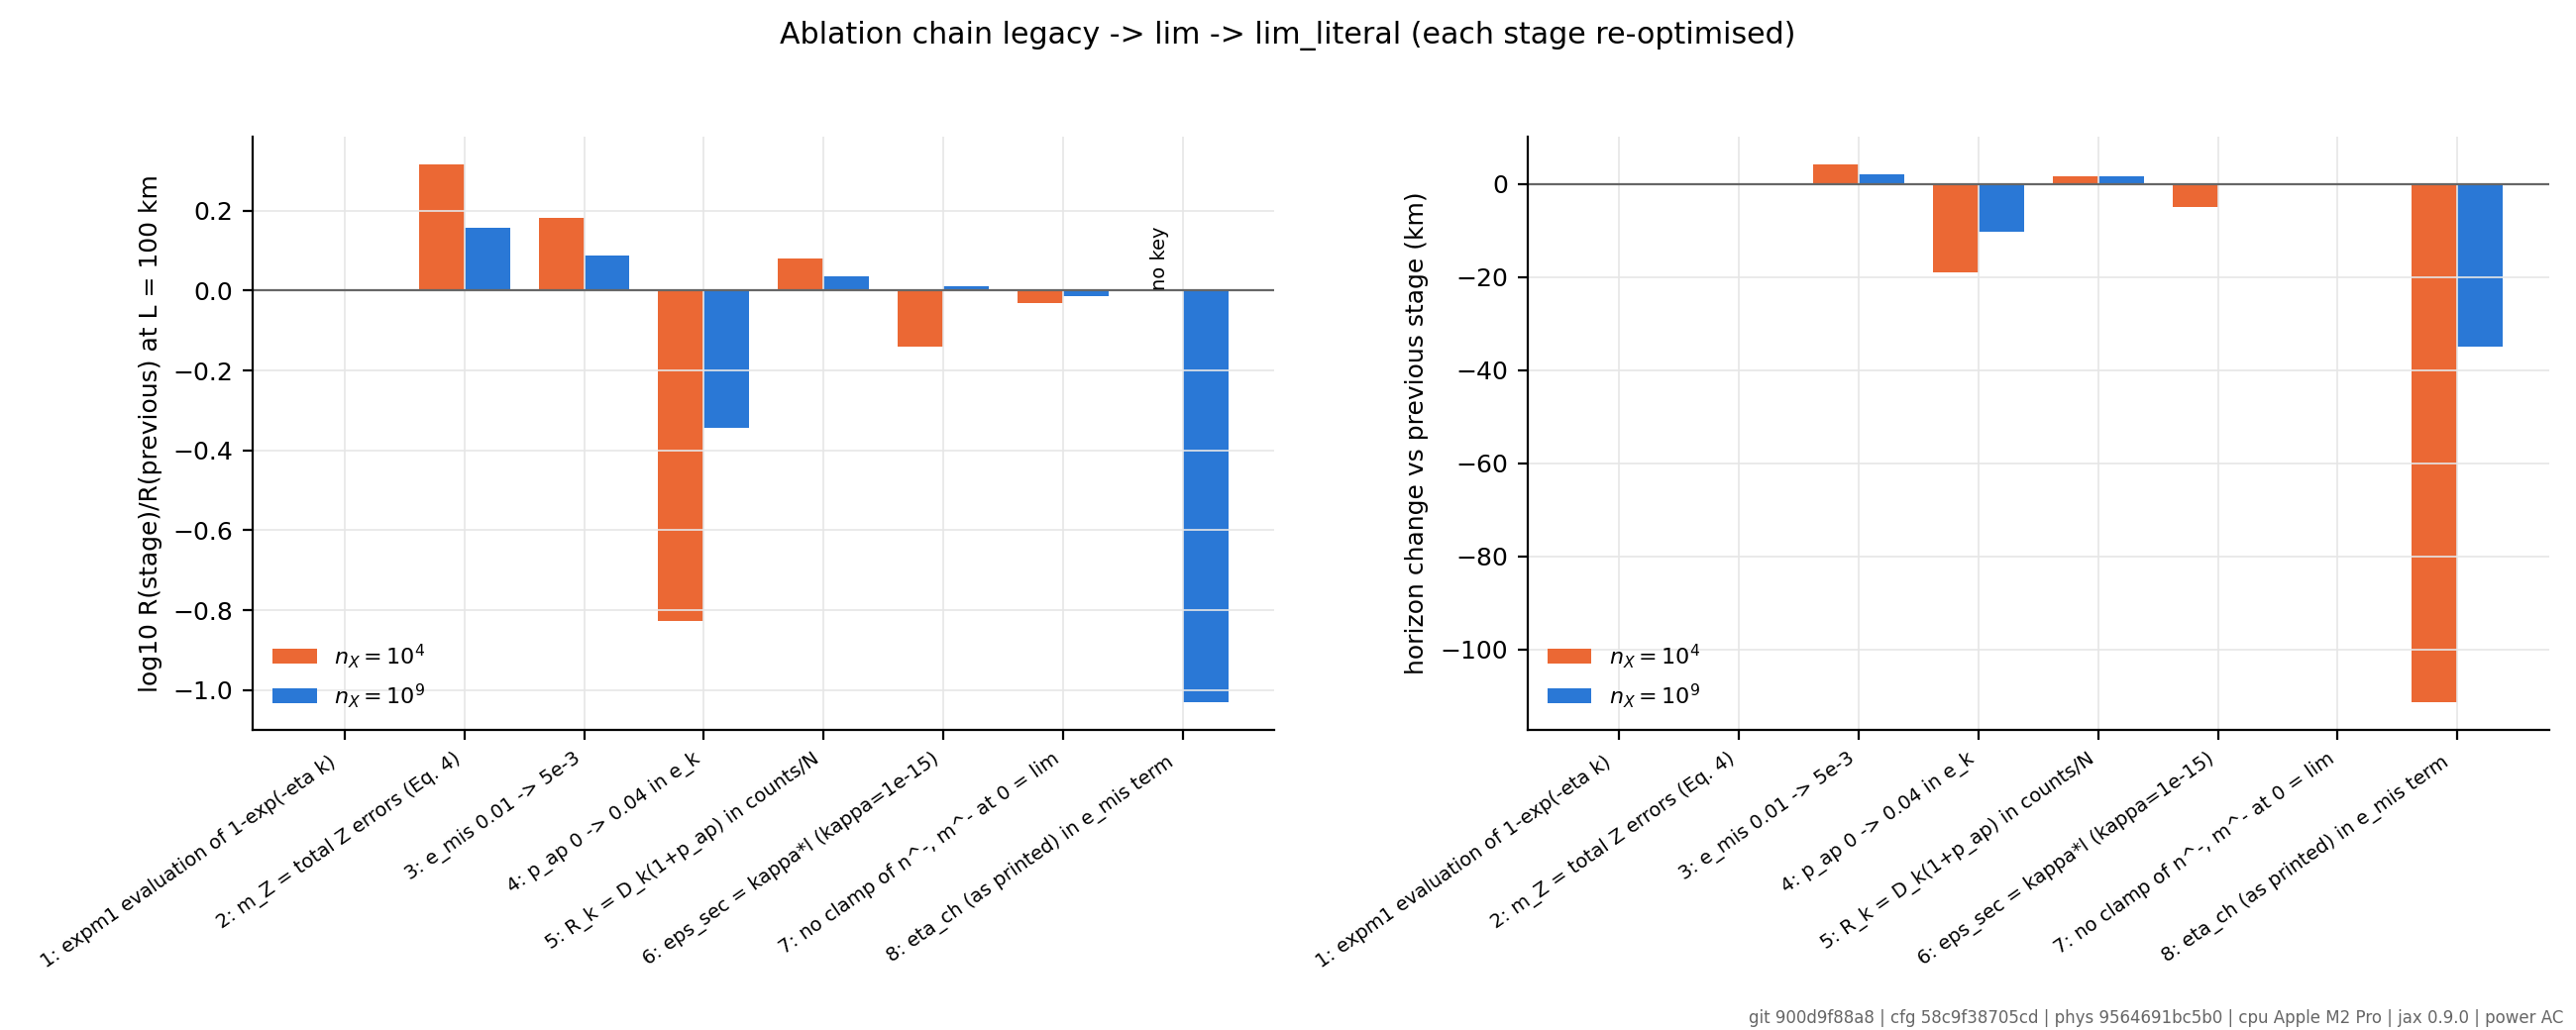
\includegraphics[width=0.9\linewidth]{fig7_ablation.png}
\caption{The ablation of Table~\ref{tab:chain} as $\Delta\log_{10}R$ at 100\,km and $\Delta$horizon (\texttt{fig7}).}
\end{figure}

\subsection{Numerical correctness}\label{sec:numerics}
\paragraph{Independent implementation.} \path{tests/test_independent_physics.py} is a float64 and Decimal
implementation written from the paper text that does not import the JAX code. With fixed $\esec=10^{-10}$ and the \plim\ switches it agrees on $\ell$ to
$1.0\times10^{-13}$\typed\ at 360 interior points. With the full \plim\ preset it agrees to $1.7\times10^{-13}$\typed\ at 18 near-horizon points, and
on the $\esec$ fixed point to $6.3\times10^{-13}$\typed. An 80-digit evaluation confirms that the error budget of
Eq.~(1) equals $21\esec$.

\paragraph{Cancellation fix.} Near the horizon, $\eta_{\mathrm{sys}}k\approx10^{-8}$, and evaluating
$1-e^{-x}$ directly loses accuracy. Because $\ell$ is a small difference of terms up to 658 times larger, this
produced a relative error in $\ell$ of up to $1.4\times10^{-8}$\typed\ against a 60-digit evaluation. With
$-\mathrm{expm1}(-x)$, a float64 implementation is within $\sim6\times10^{-14}$\typed\ of the 60-digit value. The
patched JAX preset was not re-measured against 60 digits. It agrees with that implementation to
$1.7\times10^{-13}$\typed. No horizon moved by more than
$10^{-4}$\,km.

\paragraph{The closed-form $\gamma$ is conservative.} Lim's closed-form $\gamma$ exceeds the deviation
$\theta$ obtained by solving the exact Fung--Ma--Chau tail bound for the same failure probability $a=\esec/21$, at
every point checked (we did not prove this in general). At the 105 \plim\ operating points the ratio is 1.28--1.44 (median 1.41)\typed. The exact form would extend the
$n_X=10^4$ horizon from 130.44 to 132.35\,km\typed, and moves it by at most 0.21\,km\typed\ for $n_X\ge10^6$. It
is kept as a diagnostic preset (\texttt{lim\_tight}), not as the default (Fig.~\ref{fig:gamma}).

%======================================================================
\section{Optimizer}\label{sec:optimizer}
%======================================================================
\paragraph{Feasibility by construction.} $\theta\in\mathbb{R}^5\mapsto p$ through sigmoids and nested affine maps
(\texttt{reparam.py}). These guarantee
\[
  \mu_3<\mu_2<0.5,\qquad \mu_2+\mu_3<\mu_1<0.9,\qquad P_{\mu_k}>0,\ \textstyle\sum_k P_{\mu_k}=1,\qquad 0<q_x<1 .
\]
There are no penalty terms. The earlier code used a $10^{250}$ step penalty, which has zero gradient.

\paragraph{Objective.} Where a positive key exists, the optimizer maximises $R$. Beyond the horizon, maximising
$R$ is degenerate: $R<0$ is pushed towards $0^-$ by $q_x\to0$. There the optimizer maximises $\ell/n_X$ instead,
which is smooth and has the same sign as $\max_pR$ (because $N>0$). The horizon is then exactly the zero of
$\max_p\ell$. Neither $R$ nor $\ell$ is ever clipped. The objective is divided by its value at the best start, so
tolerances are relative ($R$ spans $10^{-2}$ to $10^{-11}$).

\paragraph{Global and local stages.}
\begin{itemize}
\item \emph{Global:} scrambled Sobol points in $u$-space (mapped to $\theta$), evaluated with \texttt{jit}+\texttt{vmap}; the
  diverse top-$k$ are kept.
\item \emph{Local:} saddle-free damped Newton with the exact $5\times5$ Hessian (absolute eigenvalues,
  regularised), a step cap and Armijo backtracking, all in float64.
\item \emph{Warm sweep:} continuation along $L$. A global re-check runs every 10 points. A branch switch found by a re-check is
  logged, and the sweep backfills backwards from it. Changes between re-checks that need no switch are not
  logged (open issue~1). the horizon is refined to $\ell=0$ by bisection.
\end{itemize}

\paragraph{Certificate.} Each point is returned with:
\begin{itemize}
\item a status, e.g.\ \texttt{converged\_grad} or \texttt{no\_descent};
\item $\|\nabla_\theta\|_\infty$ of the scaled objective (objective divided by $|$value at the best start$|$);
\item the Hessian eigenvalues;
\item the active bounds;
\item a branch id.
\end{itemize}

%======================================================================
\section{Evaluation protocol}\label{sec:protocol}
%======================================================================
\subsection{Trusted reference}
\paragraph{Grids.}
\begin{itemize}
\item \emph{Bulk:} 21 fiber lengths (every 20th point of \texttt{linspace(0,200,400)} plus the last; about 10\,km
  apart; the same $L$ values as the earlier runs) $\times$ $n_X\in\{10^4,\dots,10^9\}$, i.e.\ 126 points.
\item \emph{Tail:} every 0.501\,km grid point from 15\,km below to 1\,km above each horizon, i.e.\ 192 points.
\end{itemize}

\paragraph{Construction.} For \plim\ and \limlit, each reference point is the best of four candidates:
\begin{itemize}
\item two independent cold solves ($2^{17}$ Sobol points, seeds 0/1 bulk and 2/3 tail, top 64 refined by Newton);
\item two neighbour-continuation solves, one from each side in $L$.
\end{itemize}
The \legacy\ reference uses the two Sobol solves plus Newton refinement started from the three stored earlier
runs. It was not rebuilt with continuation candidates.

\paragraph{Acceptance tests.}
\begin{enumerate}
\item The two seeds agree to $3.3\times10^{-13}$\typed\ (bulk) and $7.6\times10^{-13}$\typed\ (tail).
\item An \emph{independent} optimizer (SciPy SLSQP in $p$-space, random starts, different code path) never beats
  the reference by more than the tolerance $\mathrm{tol}_{\mathrm{ref}}=\max(10^{-9},2\times\text{seed
  disagreement})$: \QKDLimXcheckMainWeak\ weaknesses in the bulk and \QKDLimXcheckTailWeak\ in the tail.
\item $10^5$ random perturbations (scales $10^{-6}$--$10^{-1}$) around each of 72 tail points improve $R$ by at
  most $4.9\times10^{-13}$\typed.
\end{enumerate}
SLSQP itself is weaker than the reference near the horizon: it agrees within $10^{-6}$ at
\QKDLimXcheckMainPctAgree\,\% (bulk) and \QKDLimXcheckTailPctAgree\,\% (tail) of points, and is otherwise
\emph{worse}. That makes it a test the reference can fail, not one it is guaranteed to pass.

\paragraph{cliff\_edge points.} A point with $R>0$ and certificate gradient $>10^{-3}$ is labelled
\emph{cliff\_edge}. These are the last points before the horizon, where the greatest fixed point of
$\esec=\kappa\ell$ disappears and $R(p)$ is discontinuous. There, ``optimal'' is not a well-conditioned target.
Such points are excluded from scores and listed separately: 2 of 105 bulk points with $R>0$, and 5 of 180 tail
points\typed. Points with gradient between $10^{-6}$ and $10^{-3}$ (\emph{noise\_floor}) are scored. This applies to \plim\
and \limlit. The \legacy\ references were built before this rule and use the earlier threshold, $10^{-6}$. With a
fixed $\esec$, the large gradients there come from $|R|\to0$ at the horizon.

\subsection{Metrics}
\begin{description}
\item[Regret] $r=(R_{\mathrm{ref}}-R(\hat p))/R_{\mathrm{ref}}$, with $R(\hat p)$ re-evaluated by the float64
  model at the method's parameters. We report the median, p99, maximum, and the fraction with $r\le10^{-6}$
  (also $10^{-4},10^{-3},10^{-2}$). $r\ge1$ means the parameters give no key.
\item[Horizon] The largest $L$ with $\max_p\ell>0$, found by bisection. It is \emph{not} a threshold on $R$; the
  earlier $R\ge10^{-12}$ convention was arbitrary.
\item[Smoothness] Total variation per km of the box-normalised parameters on
  $S=\{L:R_{\mathrm{ref}}(L)>10^{-3}R_{\mathrm{ref}}(0)\}$. Logged branch-switch pairs are excluded and listed.
  Restricting to $S$ removes the region beyond the horizon, which dominated the earlier roughness numbers.
\item[Timing] Wall-clock time on one machine (Apple M2 Pro, CPU backend, float64, JAX 0.9.0, AC power, no other
  jobs). JIT compile time is reported separately. Device-resident and end-to-end medians are both given, and every
  timing names its batch size and warm or cold start.
\end{description}

%======================================================================
\section{Results}\label{sec:results}
%======================================================================
\subsection{Horizons and key rate}
\begin{table}[H]\centering\small
\begin{tabular}{lcccccc}\toprule
Preset & $10^4$ & $10^5$ & $10^6$ & $10^7$ & $10^8$ & $10^9$\\\midrule
\plim   & \QKDLimRefHorizonFour & \QKDLimRefHorizonFive & \QKDLimRefHorizonSix & \QKDLimRefHorizonSeven & \QKDLimRefHorizonEight & \QKDLimRefHorizonNine\\
\limlit & \QKDLimLiteralRefHorizonFour & \QKDLimLiteralRefHorizonFive & \QKDLimLiteralRefHorizonSix & \QKDLimLiteralRefHorizonSeven & \QKDLimLiteralRefHorizonEight & \QKDLimLiteralRefHorizonNine\\
\legacy & \QKDLegacyRefHorizonFour & \QKDLegacyRefHorizonFive & \QKDLegacyRefHorizonSix & \QKDLegacyRefHorizonSeven & \QKDLegacyRefHorizonEight & \QKDLegacyRefHorizonNine\\\bottomrule
\end{tabular}
\caption{Reference horizons (km) for each $n_X$. The new warm sweep reproduces the \plim\ horizons to within
0.0072\,km\typed.}\label{tab:horizons}
\end{table}

\begin{figure}[H]\centering
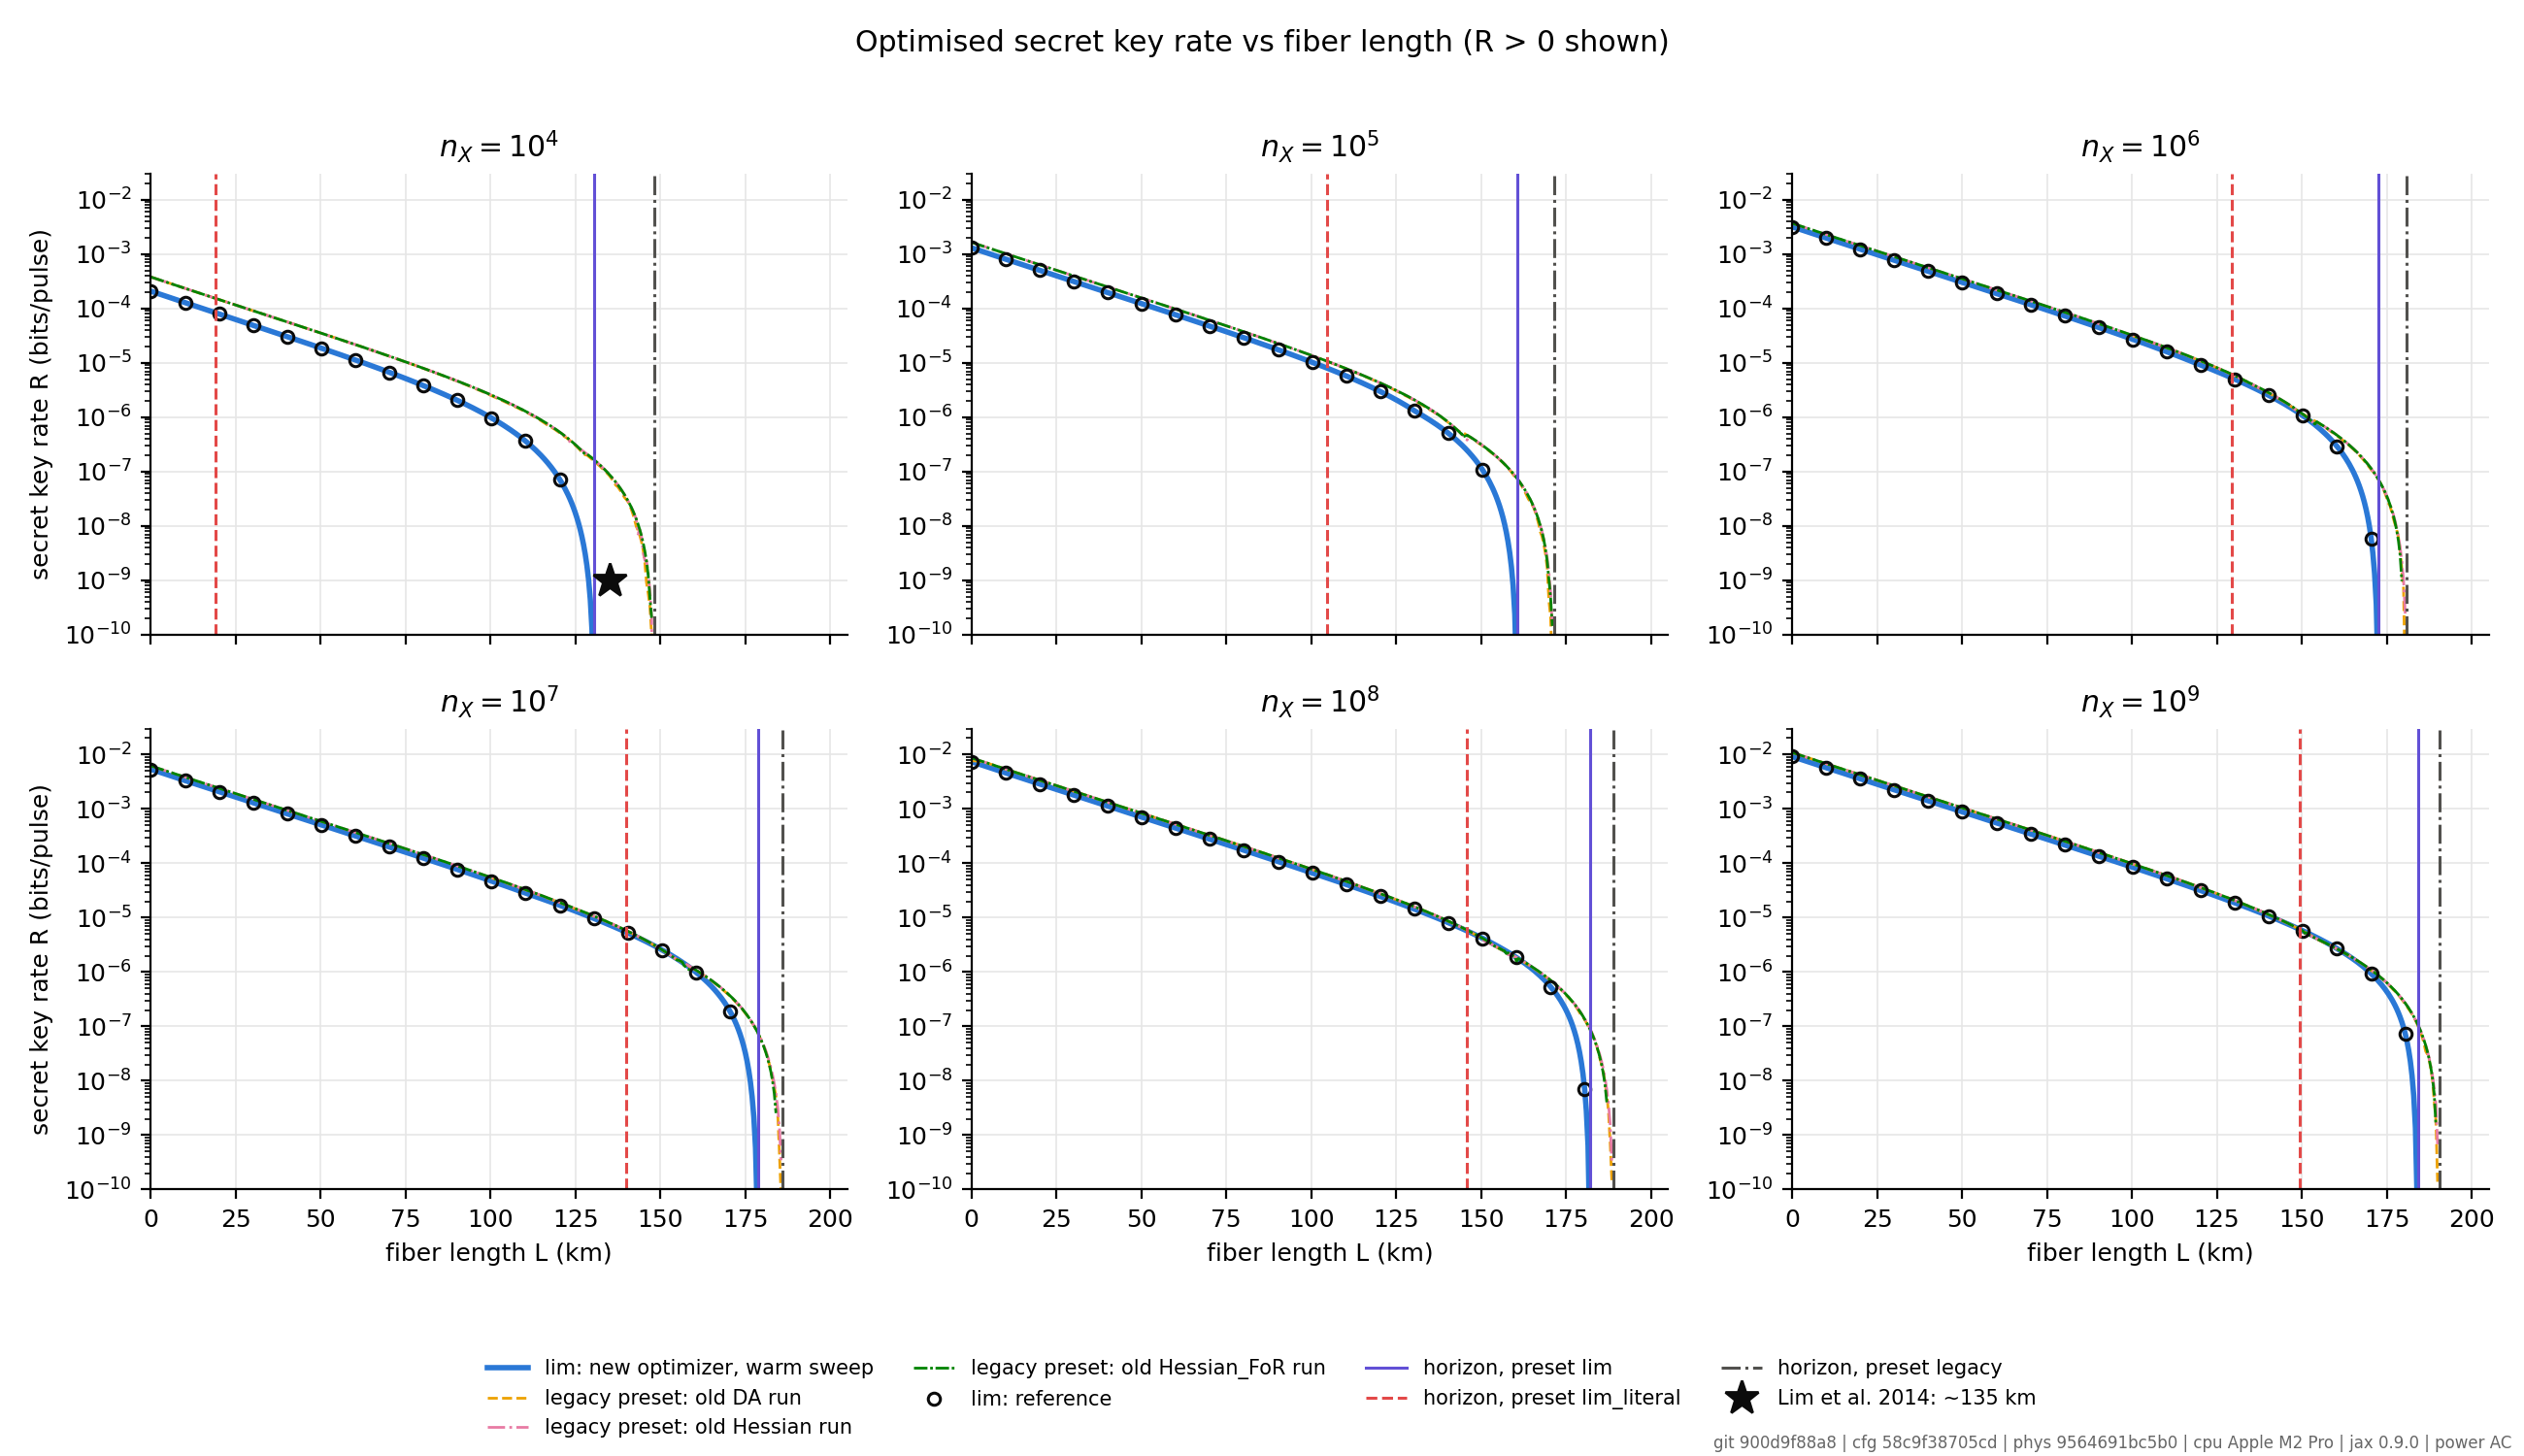
\includegraphics[width=\linewidth]{fig1_keyrate.png}
\caption{Optimal key rate under \plim\ (warm sweep and reference points), with the stored earlier runs evaluated
under \legacy, the objective they were optimised for (\texttt{fig1}).}
\end{figure}

\subsection{Accuracy of the optimal parameters and key rates}
\begin{table}[H]\centering\small
\fitbox{\begin{tabular}{llccc}\toprule
Preset & Method & \% $r\le10^{-6}$ (bulk / tail) & median $r$ (bulk) & max $r$ (bulk / tail)\\\midrule
\plim & new, cold start & \QKDLimNewColdPctWithin\ / \QKDLimTailNewColdPctWithin & \QKDLimNewColdRegretMedian & \QKDLimNewColdRegretMax\ / \QKDLimTailNewColdRegretMax\\
\plim & new, warm sweep & \QKDLimNewWarmPctWithin\ / \QKDLimTailNewWarmPctWithin & \QKDLimNewWarmRegretMedian & \QKDLimNewWarmRegretMax\ / \QKDLimTailNewWarmRegretMax\\
\plim & lookup table (2\,km nodes) & \QKDLimLookupPctWithin\ / \QKDLimTailLookupPctWithin & \QKDLimLookupRegretMedian & \QKDLimLookupRegretMax\ / \QKDLimTailLookupRegretMax\\\midrule
\legacy & new, warm sweep & \QKDLegacyNewWarmPctWithin\ / \QKDLegacyTailNewWarmPctWithin & \QKDLegacyNewWarmRegretMedian & \QKDLegacyNewWarmRegretMax\ / \QKDLegacyTailNewWarmRegretMax\\
\legacy & earlier DA run & \QKDLegacyOldDAPctWithin\ / \QKDLegacyTailOldDAPctWithin & \QKDLegacyOldDARegretMedian & \QKDLegacyOldDARegretMax\ / \QKDLegacyTailOldDARegretMax\\
\legacy & earlier Hessian run & \QKDLegacyOldHessianPctWithin\ / \QKDLegacyTailOldHessianPctWithin & \QKDLegacyOldHessianRegretMedian & \QKDLegacyOldHessianRegretMax\ / \QKDLegacyTailOldHessianRegretMax\\
\legacy & earlier Hessian\_FoR run (NN labels) & \QKDLegacyOldFoRPctWithin\ / \QKDLegacyTailOldFoRPctWithin & \QKDLegacyOldFoRRegretMedian & \QKDLegacyOldFoRRegretMax\ / \QKDLegacyTailOldFoRRegretMax\\\bottomrule
\end{tabular}}
\caption[Regret against the trusted reference]{Regret against the trusted reference, with cliff\_edge points excluded (bulk: 103 \plim\ / 109 \legacy\
points; tail: 175 / 142; the \legacy\ counts use the earlier cliff\_edge threshold)\typed. The earlier runs are scored on their own objective (\legacy). The cold start
uses Sobol seed 7, independent of the reference seeds. The lookup table interpolates the new optimizer's own optima
linearly in $L$ between nodes 2\,km apart, separately for each $n_X$; it is the simplest surrogate and the floor for Section~\ref{sec:qml}.
Regret above 1 means the parameters yield no key.}\label{tab:regret}
\end{table}

\paragraph{Reading.} On \plim, the new optimizer is at the reference to $10^{-12}$ or better everywhere,
including the near-horizon tail, where the earlier DA and Hessian\_FoR runs were within $10^{-6}$ at 0\,\% of
points. The run that produced the earlier
neural-network labels missed the optimum by more than $10^{-6}$ at 18\,\% of bulk points and at every tail point.
Its worst bulk regret of 96 means a negative key rate. Any surrogate trained on those labels inherits these
errors.

\begin{figure}[H]\centering
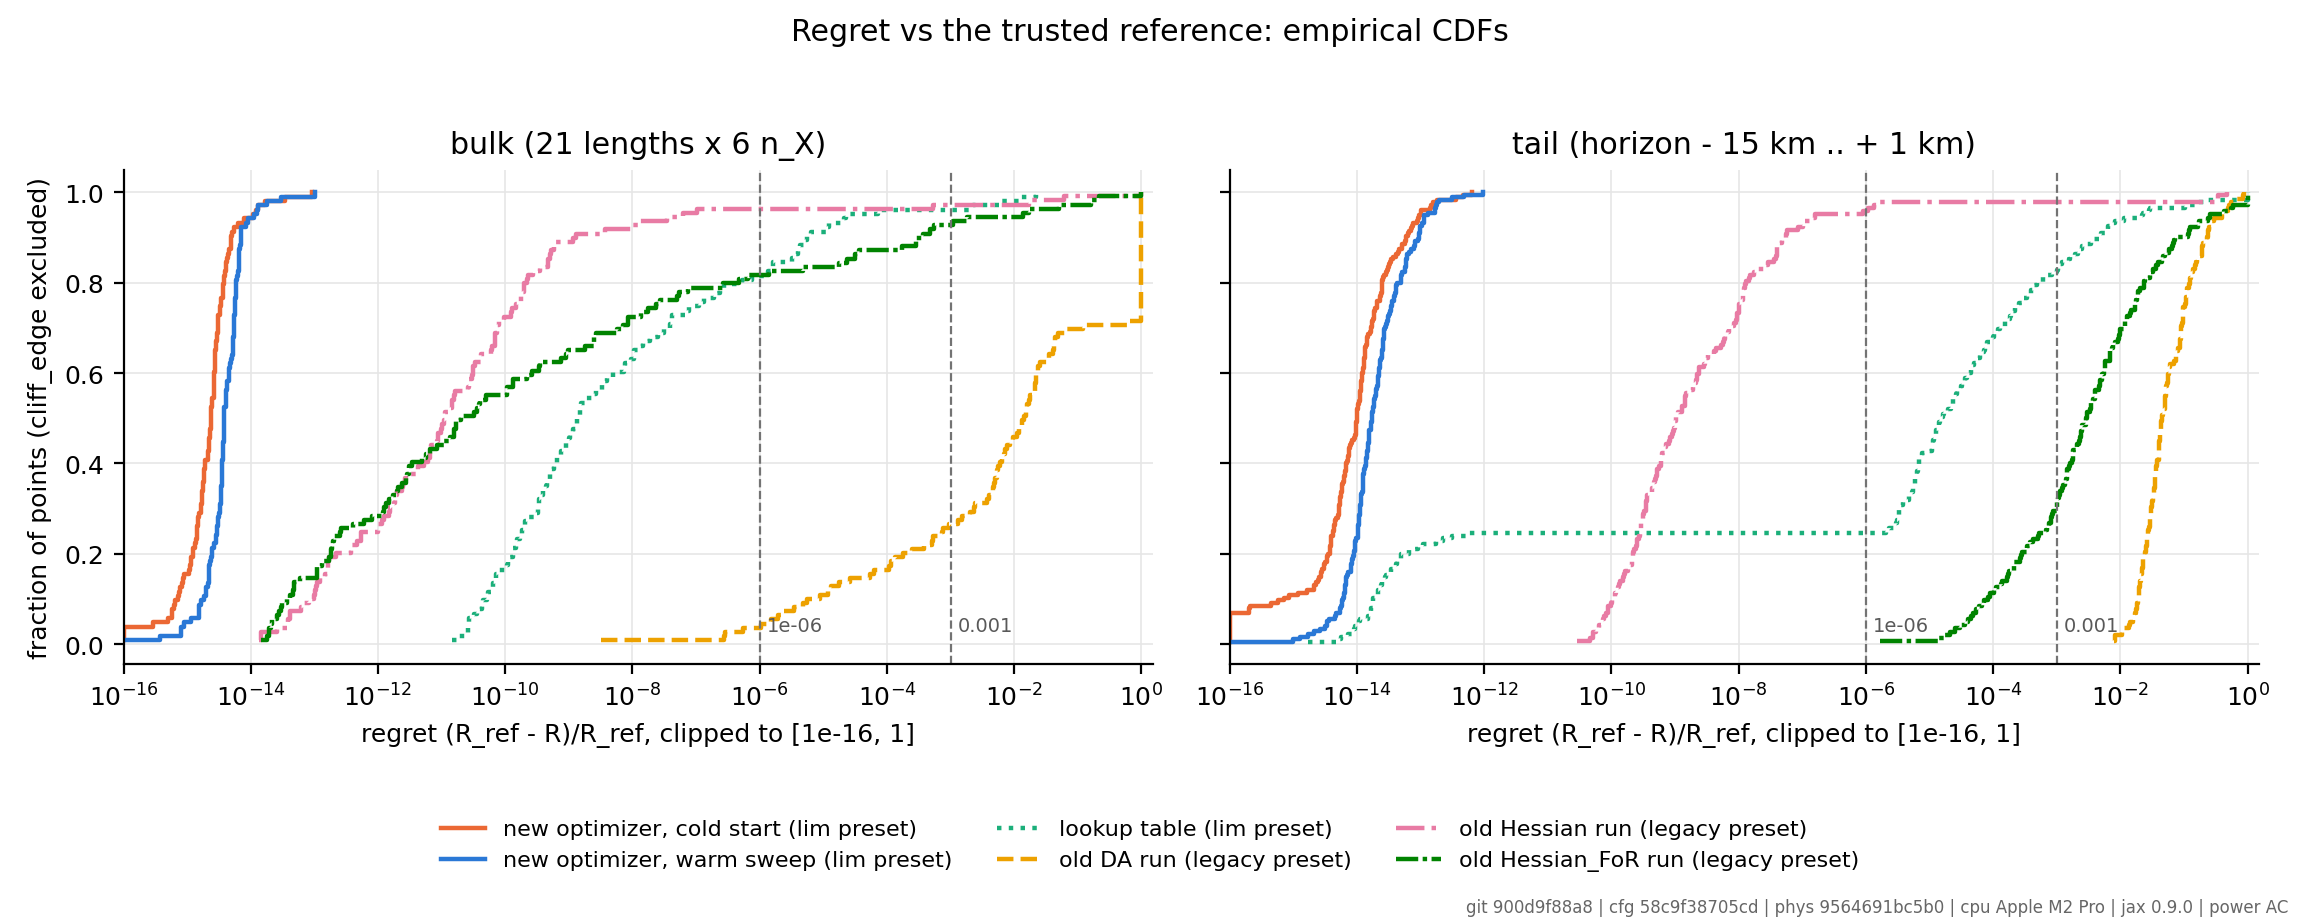
\includegraphics[width=\linewidth]{fig6_regret_cdf.png}
\caption{Empirical CDF of regret, bulk and tail (\texttt{fig6}).}
\end{figure}

\subsection{Structure of the optimal parameters}
\paragraph{Branch switches.} The stored earlier runs jump repeatedly between 148 and 157\,km at
$n_X=10^9$\typed:
\begin{itemize}
\item DA: 5 jumps;
\item Hessian\_FoR: 5 jumps;
\item Hessian: 1 jump.
\end{itemize}
For \plim, the warm sweep logged two switches between competing local optima while the key is positive
(\path{results/benchmark_lim_*/summary.json}, \texttt{sweep\_events})\typed:
\begin{itemize}
\item $n_X=10^5$: detected at 135.3\,km, where the warm path was 7.7\,\% below the global candidate, with
  $u$-distance 0.068. Backfill located the crossover at 130.3--130.8\,km.
\item $n_X=10^6$: detected at 120.3\,km, with a 0.6\,\% gain and $u$-distance 0.029. Crossover at
  118.3--118.8\,km.
\end{itemize}
After backfill the sweep is on the better branch on both sides; this is why it scores 100\,\% in
Table~\ref{tab:regret}. At such a crossover the optimal parameters are genuinely discontinuous in $L$, while $R$
is continuous.

No switch was logged below the horizon for $n_X=10^4$, $10^7$, $10^8$ and $10^9$. All other logged switches
lie beyond the horizon ($R\le0$, objective $\ell/n_X$).

A dense 1\,km scan flags parameter changes larger than 0.05 (normalised) only in the last $\sim$5\,km before
each horizon. Refined to 0.1\,km, the largest step is 11--12\,\% of the 1\,km change below the horizon,
i.e.\ continuous drift. For pairs that cross the horizon it is 16--54\,\%. The dense scan did not flag the two
switches above. Their relation to the scan's threshold and normalisation has not been investigated (open
issue~6).

\paragraph{Smoothness.} TV/km on $S$, with logged switches excluded:
\begin{itemize}
\item \plim\ warm sweep: \QKDLimNewWarmTVFour\ ($n_X=10^4$) and \QKDLimNewWarmTVNine\ ($10^9$).
\item \legacy, $n_X=10^4$: new warm sweep \QKDLegacyNewWarmTVFour; earlier DA \QKDLegacyOldDATVFour\ (4.3$\times$
  rougher); earlier Hessian\_FoR \QKDLegacyOldFoRTVFour; earlier Hessian $1.85\times10^{-3}$\typed.
\item \legacy, $n_X=10^9$: new warm sweep \QKDLegacyNewWarmTVNine; earlier DA \QKDLegacyOldDATVNine\
  (1.4$\times$ rougher); earlier Hessian\_FoR \QKDLegacyOldFoRTVNine; earlier Hessian $1.84\times10^{-3}$\typed.
\end{itemize}
On the region with a useful key, the new optimizer is as smooth as the earlier Hessian-based runs and smoother
than DA. Smoothness is therefore not where it improves. The improvement is optimality: Table~\ref{tab:regret},
especially in the tail. The earlier ``$129\times$ stability'' figure came from the region beyond the horizon and is
withdrawn.

\paragraph{Note on comparing parameter values.} In Fig.~\ref{fig:params} the \plim\ curves and the earlier runs
optimise different physics, so their parameter \emph{values} are not comparable. Only continuity is compared.

\begin{figure}[H]\centering
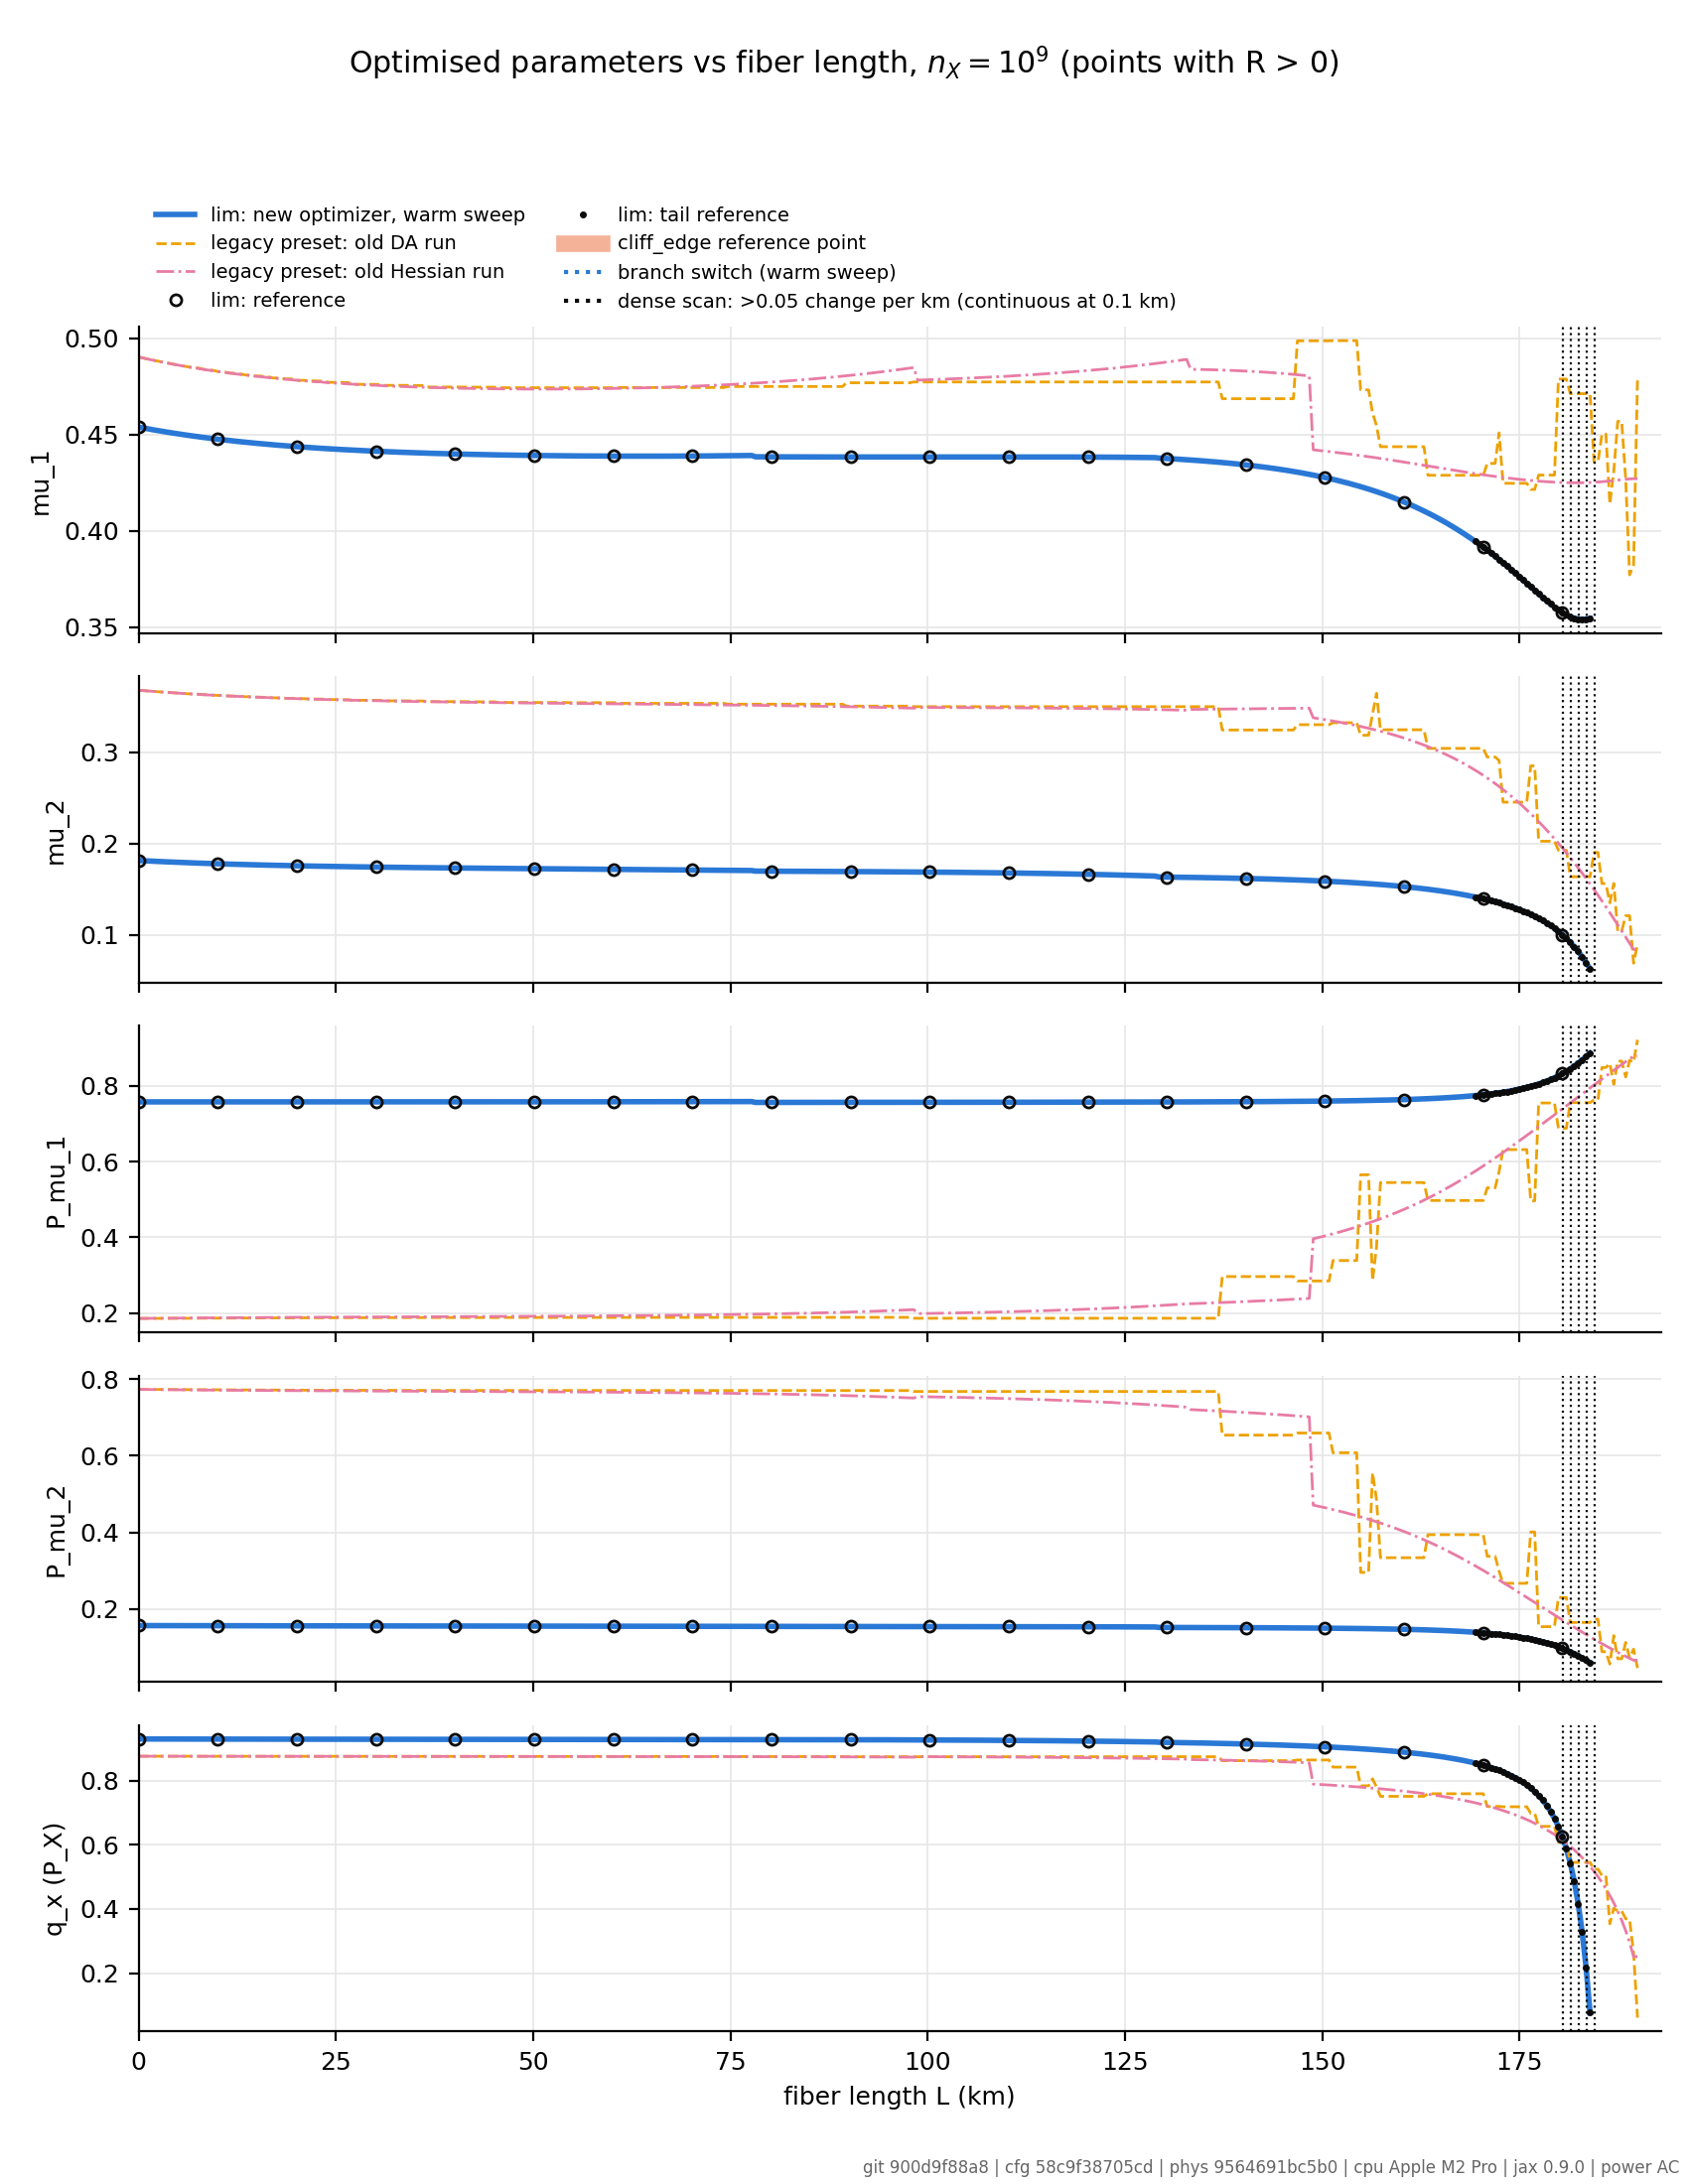
\includegraphics[width=0.74\linewidth]{fig4_params_nx1e9.png}
\caption{Optimal parameters vs $L$ at $n_X=10^9$ (\texttt{fig4}; the $n_X=10^4$ panel is
\texttt{fig4\_params\_nx1e4.png}).}\label{fig:params}
\end{figure}

\begin{figure}[H]\centering
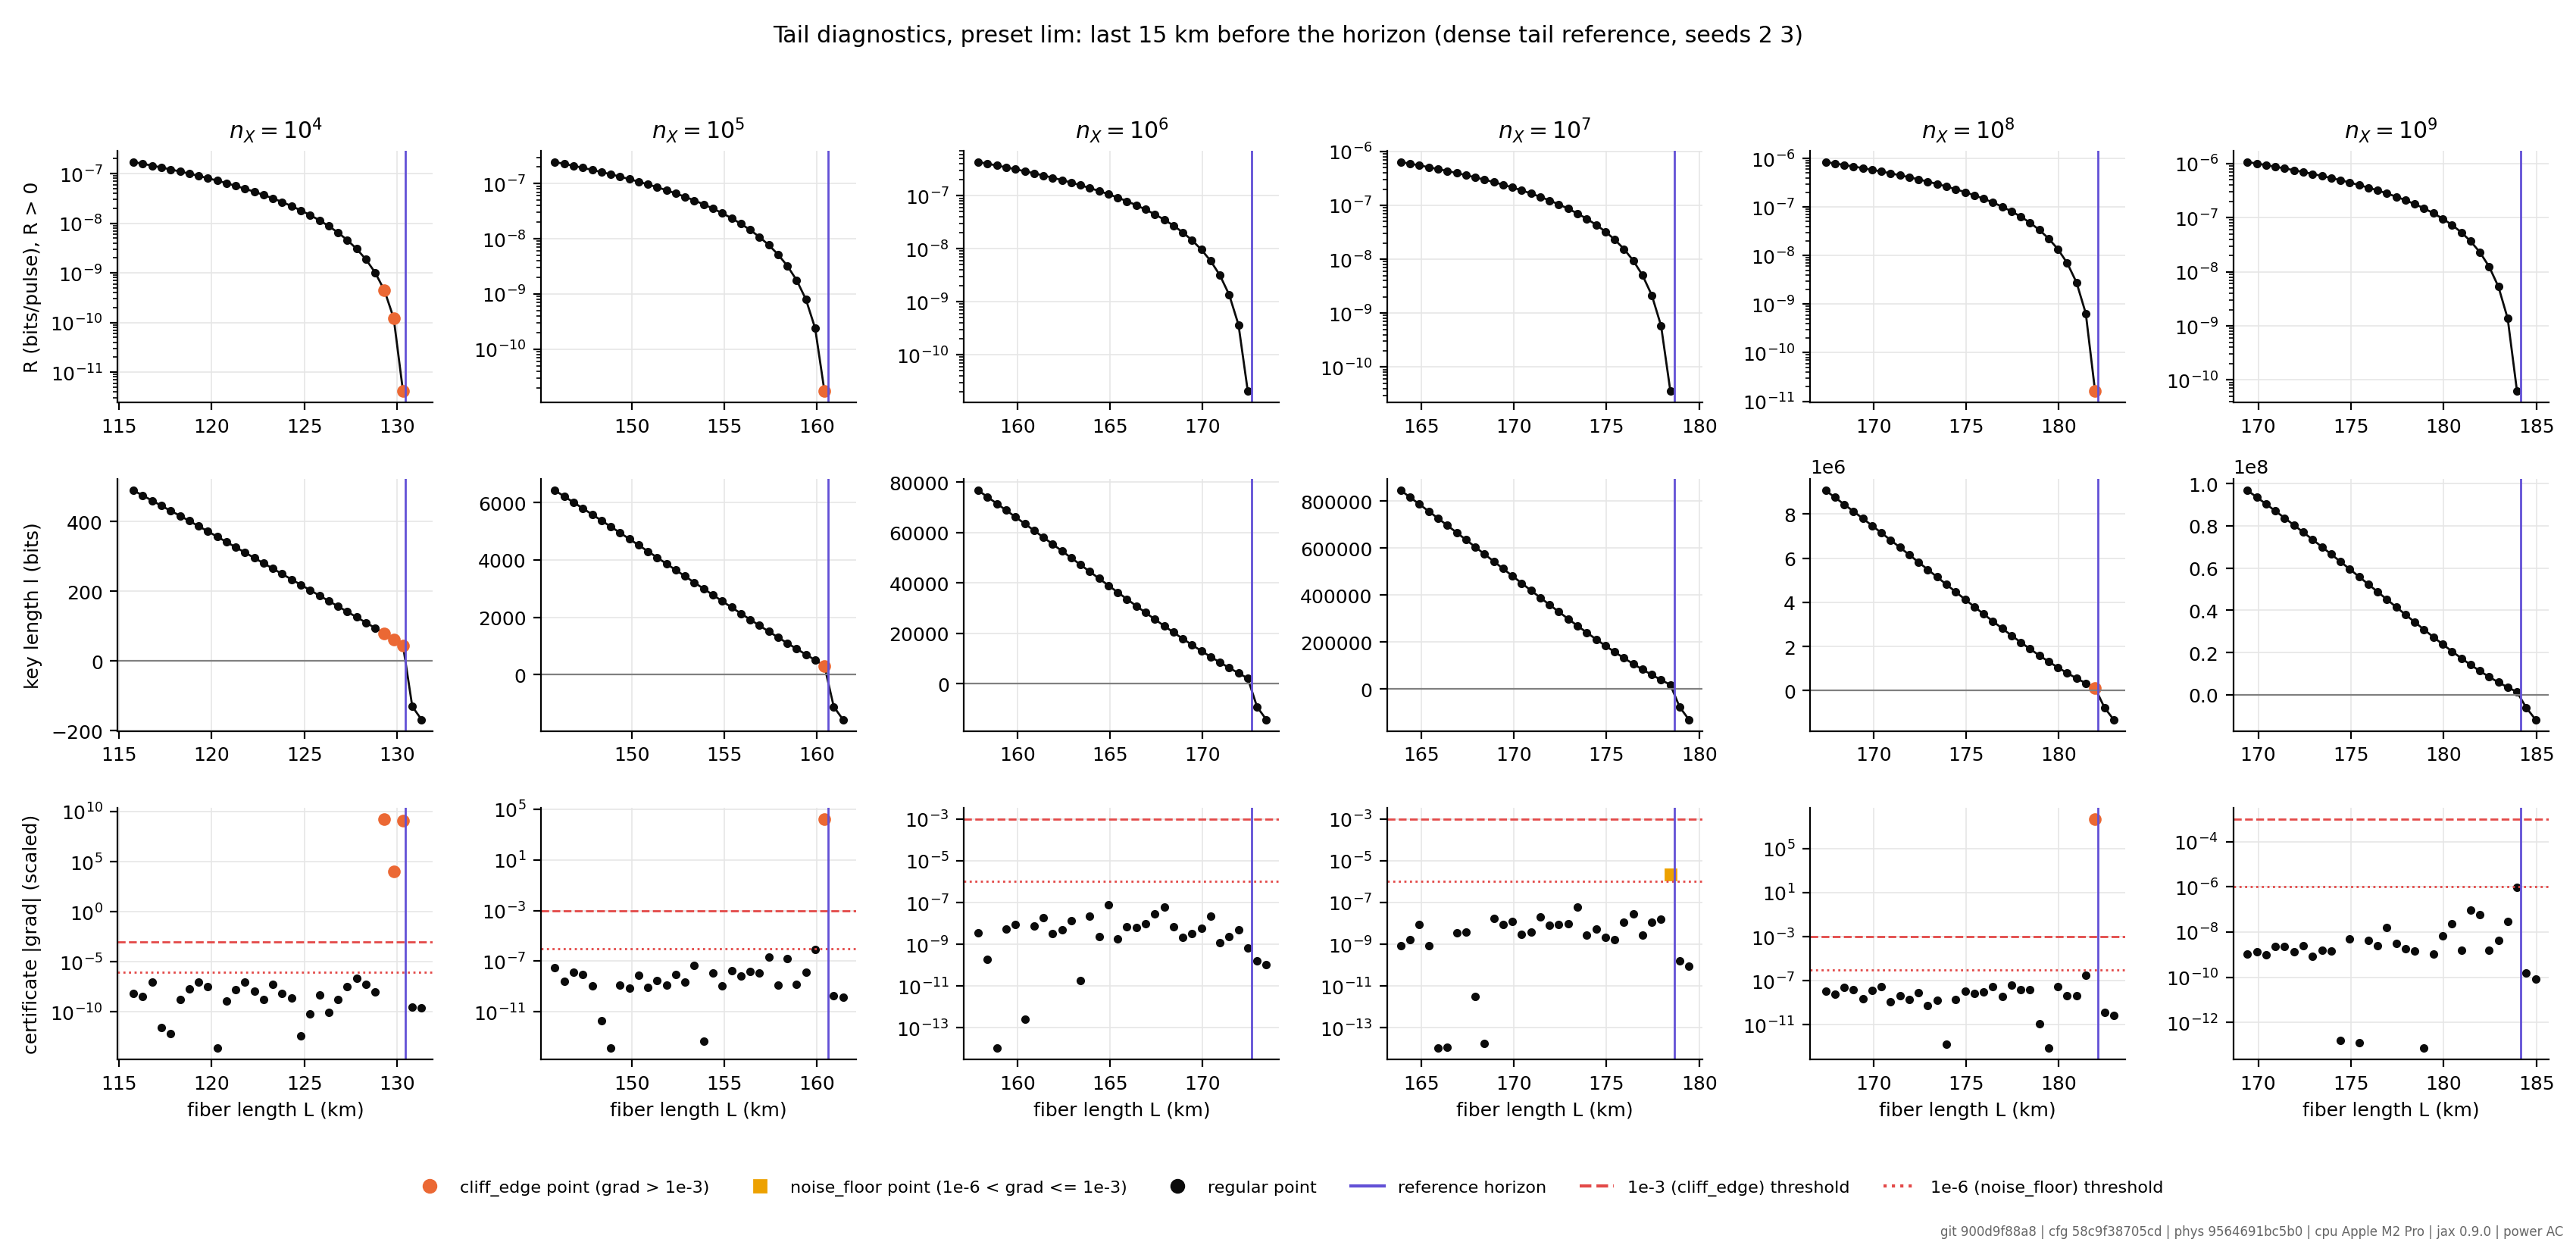
\includegraphics[width=\linewidth]{fig5_tail.png}
\caption{The last 15\,km before each horizon: $R$, $\ell$ and the certificate gradient. Orange: cliff\_edge;
yellow: noise\_floor (\texttt{fig5}).}
\end{figure}

\subsection{Computational cost}
\begin{table}[H]\centering\small
\fitbox{\begin{tabular}{lllc}\toprule
Method & start & batch & time per point\\\midrule
Earlier pipeline, $L\le100$\,km branch (L-BFGS-B) & cold & 1 & 0.7--10 ms\typed\\
Earlier pipeline, $L>100$\,km branch (DA, \texttt{maxiter} 5000--15000, 50k--150k evaluations) & cold & 1 & \QKDLimDASecMin--\QKDLimDASecMax\ s\\
New optimizer, $2^{12}$ Sobol + Newton & cold & 126 (vectorised) & 40.0 ms\typed\ (compile 38.4 s\typed)\\
New optimizer, full sweep of 2400 points & warm & 6 chains & \QKDLimSweepMsPerPoint\ ms (compile \QKDLimSweepCompileS\ s)\\
New optimizer, 100\,km, $n_X=10^9$ & warm (0.5 km away) & 1 & \QKDLimWarmDeviceUs\ $\mu$s device / \QKDLimWarmEndToEndUs\ $\mu$s end-to-end\\
New optimizer, 5\,km below each horizon & warm & 1 & 1.7--2.6 ms\typed\ device\\
Lookup table (timing variant: 2.5\,km $\times$ $\log n_X$ grid) & -- & 1 & \QKDLimLookupDeviceUs\ $\mu$s device / \QKDLimLookupEndToEndUs\ $\mu$s end-to-end\\\bottomrule
\end{tabular}}
\caption[Measured wall time]{Measured wall time on the \plim\ objective, single machine (\path{results/timing_lim_*},
\path{results/benchmark_lim_*}).}\label{tab:timing}
\end{table}
\paragraph{Fair comparisons.}
\begin{itemize}
\item \textbf{Cold vs cold:} a DA call (one point) against the new cold solver (amortised over a vectorised batch)
  is a factor of about 150--440. A batch-1 cold solve was not timed.
\item \textbf{Warm solve vs the earlier pipeline at the same distances.} Below 100\,km the earlier pipeline used
  L-BFGS-B (3.9\,ms\typed\ at 100\,km, $n_X=10^9$), only about $3\times$ slower than the warm solve, and not
  optimal. Above 100\,km it used DA. At the timed DA points where the reference has a positive key (110 and
  150\,km at $n_X=10^9$; 130\,km at $10^4$, where DA itself returned $R\le0$; 5.8--11.7\,s\typed), a warm solve (1.2--2.6\,ms) is about $2\times10^3$--$10^4$ times faster. The
  17.6\,s DA point (190\,km) lies beyond the horizon. The warm solve uses a solution 0.5\,km away, prior
  information that DA did not have.
\item \textbf{Quality:} the new solver is within $10^{-6}$ at 100\,\% of points, against
  \QKDLegacyOldDAPctWithin\,\% for the earlier DA run.
\item The lookup-table latency is measured on a slightly different table (2.5\,km nodes, interpolated also in
  $\log n_X$) from the one scored in Table~\ref{tab:regret}. Both are $O(10)\,\mu$s.
\end{itemize}
These ratios replace the withdrawn $5.9\times10^6$, $3{,}574\times$ and $270\times$ figures.

\begin{figure}[H]\centering
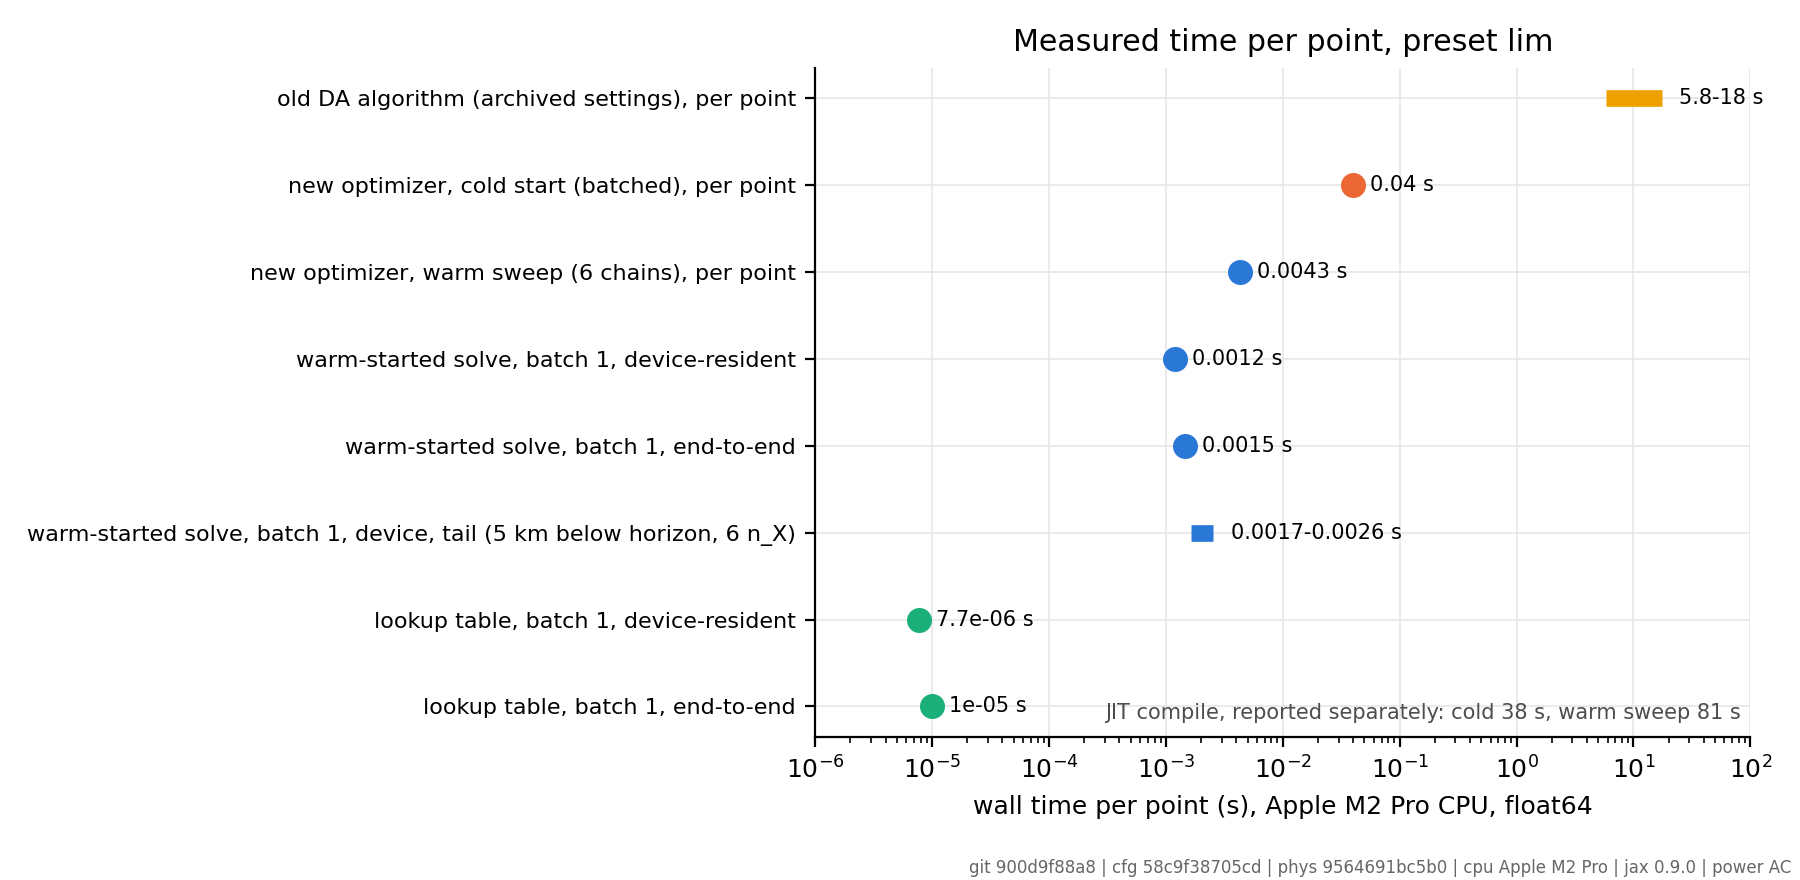
\includegraphics[width=0.8\linewidth]{fig8_timing.png}
\caption{Measured wall time per point (\texttt{fig8}).}\label{fig:timing}
\end{figure}

%======================================================================
\section{Discussion}\label{sec:discussion}
%======================================================================
\subsection{What changed relative to the earlier work}
\begin{enumerate}
\item \textbf{The model.} The earlier key rate contained a defect ($m_Z$) and departed from the paper in four
  settings (Table~\ref{tab:chain}). Its $n_X=10^4$ horizon (148.2\,km) was 17.7\,km longer than that of the
  corrected model (130.4\,km). The corrected model's horizon is 3\,\% below the paper's $\sim$135\,km.
\item \textbf{The labels.} Optimal parameters are now certified, not assumed. The earlier labels were
  sub-optimal at 18\,\% of bulk points and at all tail points, so the earlier NN accuracy figures measured
  agreement with sub-optimal targets.
\item \textbf{The metrics.} Regret on re-evaluated $R$ replaces relative parameter error. The horizon is
  $\ell=0$ instead of $R\ge10^{-12}$. Smoothness excludes the no-key region. Timings compare equal work and state
  batch size and warm or cold start.
\end{enumerate}

\subsection{Threats to validity}
\begin{enumerate}
\item \textbf{Model fidelity.} \plim\ matches the paper to within 8\,\%, not exactly, and rests on the choices in
  Section~\ref{sec:choices}. Using $\eta_{\mathrm{sys}}$ instead of the printed $\eta_{\mathrm{ch}}$ is an
  inference from Table~\ref{tab:targets}. All results are conditional on this model. Changing it changes the
  numbers but not the method.
\item \textbf{Expected counts.} Observed counts are set to their expectations (a choice the paper does not
  print), so statistical fluctuations of an actual run are not modelled.
\item \textbf{Continuous relaxation.} Dropping the floor in Eq.~(1) changes $\ell$ by less than one bit, i.e.\
  relatively by at most $1/\ell$. That is negligible in the bulk and about 2\,\% at the smallest cliff\_edge keys
  ($\ell\approx45$ bits).
\item \textbf{The reference is the best known optimum, not a proof of global optimality.} The evidence for it is:
  \begin{itemize}
  \item two independent seeds;
  \item an independent optimizer (SLSQP) on a different code path;
  \item a local perturbation test.
  \end{itemize}
  The reference and the new optimizer share the physics and the Newton solver. The physics is checked
  independently (Section~\ref{sec:numerics}); the SLSQP cross-check is the independent check on the optimisation.
\item \textbf{Excluded points.} The cliff\_edge exclusions (2 bulk, 5 tail) remove points where $R(p)$ is
  discontinuous. Scores there are listed separately, not hidden.
\item \textbf{The earlier runs scored here} are the February 2026 script outputs. The 2025 thesis dataset and
  network were not re-scored (Appendix~\ref{app:supersede}).
\item \textbf{Timing} comes from one CPU machine; GPU and other hardware were not measured.
\end{enumerate}

\subsection{Open issues}
None of these affects the \plim\ results above (from \texttt{STATUS.md}):
\begin{enumerate}
\item A $\sim$0.002 (normalised) parameter step at $n_X=10^9$, 77.7--78.2\,km, is not logged as an event; $R$ is
  smooth there. Proposed fix: a \texttt{drift\_step} log.
\item \limlit\ tail (diagnostic): the new optimizer misses the reference by up to
  \QKDLimLiteralTailNewColdRegretMax\ at 3 of 146 points. Not yet investigated.
\item \legacy\ tail: one cold-start point has regret \QKDLegacyTailNewColdRegretMax. The \legacy\ references were
  not rebuilt with continuation candidates.
\item The sensitivity, robustness and extrapolation analyses (\texttt{analyses.py}) have not been re-run since the
  expm1 fix.
\item The neural network has not been retrained (\texttt{NN\_RETRAIN\_PLAN.md}).
\item The two below-horizon branch switches ($n_X=10^5$, $10^6$) were found by the sweep but not by the dense
  scan. Characterise both optima there, and make the scan sensitive to switches of this size.
\end{enumerate}

%======================================================================
\section{Benchmark protocol for surrogates (classical NN and QML)}\label{sec:qml}
%======================================================================
The value of a surrogate is a trade-off between \emph{regret} and \emph{latency}. The protocol below is fixed
\emph{before} any model is trained, so that the classical and quantum models are compared on identical terms. It
encodes the lessons of the earlier work.

\paragraph{Task.} Learn $x\mapsto p^\star(x)$ with $x=(L,\log_{10}n_X)$, optionally extended by
$p_{\mathrm{dc}}$, $e_{\mathrm{mis}}$ and $\alpha$ (ranges in \texttt{NN\_RETRAIN\_PLAN.md}). Models predict in
$\theta$- or $u$-space, so that every prediction is feasible by construction.

\paragraph{Labels.}
\begin{itemize}
\item Generated where compute is cheap (e.g.\ cloud CPU/GPU), not on a laptop.
\item Generated by the new optimizer under \plim\ (or under the extended model, with the same verification).
\item Each label carries its certificate.
\item cliff\_edge points are excluded from training and from scoring, and listed. Near the two crossovers
  (118.5 and 130.5\,km), $p^\star$ is discontinuous. Report them separately.
\end{itemize}

\paragraph{Splits (no test point on the training grid).}
\begin{itemize}
\item \emph{Interpolation:} held-out $L$ between training nodes, and held-out block sizes (e.g.\
  $n_X=5\times10^8$, as in the thesis).
\item \emph{Tail:} the dense tail grid, scored separately.
\item \emph{Extrapolation:} reported separately, never pooled with interpolation.
\end{itemize}

\paragraph{Primary metric.} Regret of the float64 $R$ re-evaluated at the predicted parameters, reported for bulk
and tail separately:
\begin{itemize}
\item the median, p99 and maximum;
\item the fractions with $r\le10^{-6}$, $10^{-4}$, $10^{-3}$ and $10^{-2}$;
\item the fraction with no key ($r\ge1$).
\end{itemize}
Secondary metrics: horizon error, and parameter error in $u$-space. Parameter error alone is not sufficient
because $R$ is flat in some directions and steep in others.

\paragraph{Baselines.} A surrogate is compared against three references:
\begin{enumerate}
\item the lookup table: \QKDLimLookupPctWithin\,\% (bulk) and \QKDLimTailLookupPctWithin\,\% (tail) within
  $10^{-6}$, at \QKDLimLookupEndToEndUs\,$\mu$s;
\item a classical NN with a matched parameter count;
\item the warm-started exact solver: 100\,\% within $10^{-6}$, at \QKDLimWarmEndToEndUs\,$\mu$s.
\end{enumerate}
We also report the hybrid ``surrogate prediction + $k$ Newton steps'' for $k=1,2,3$. Whether it beats both
components has not been measured.

\paragraph{Cost accounting.}
\begin{itemize}
\item Latency: batch-1 end-to-end and device-resident, plus batched throughput.
\item Training cost.
\item For QML: the backend (simulator or hardware), the shots per prediction and the circuit evaluations per
  prediction. On hardware these dominate latency and must not be omitted.
\end{itemize}

\paragraph{Statistics.} At least 5 training seeds, reported as mean $\pm$ standard deviation. Hyperparameters are
chosen on a validation split, never on the test split.

\paragraph{Usefulness criterion.} A surrogate is useful if either of the following holds:
\begin{itemize}
\item it reaches the warm solver's regret class at lower latency;
\item it beats the lookup table's regret at comparable latency.
\end{itemize}
Every comparison in the QML project should be framed against this criterion.

\paragraph{Amendment 1 (2026-11-06).} The sentence under \emph{Labels} above (``Generated where compute is cheap
(e.g.\ cloud CPU/GPU), not on a laptop'') is left unchanged. For the PQC surrogate study (branch
\texttt{qml-surrogate}, \path{qml/PREREGISTRATION.md}), labels are instead generated locally on AC power, because
the measured cost is small: 4.27\,ms per point for the warm sweep plus an 81\,s one-time compile, and about
40\,ms per point for a cold solve (\path{results/benchmark_lim_0c8f47a1f0_530f6d58460c/summary.json}).

%======================================================================
\section{Conclusion}
%======================================================================
The parameter-optimisation problem for finite-key decoy-state BB84 is now solved to within $10^{-12}$ relative
regret of an independently cross-checked best-known reference (cliff\_edge points excluded), on a corrected model which is validated against the paper and against an independent implementation:
\begin{itemize}
\item the optimal parameters vary smoothly with distance, apart from two logged switches between competing optima;
\item the horizons and key rates are reproducible from scripts with recorded provenance;
\item the earlier speed-up, stability and neural-network claims are withdrawn.
\end{itemize}
The reference, metrics and protocol of Sections~\ref{sec:protocol} and~\ref{sec:qml} are the basis for the
classical-versus-quantum surrogate benchmark.

%======================================================================
\appendix
\section{Earlier documents and their status}\label{app:supersede}
%======================================================================
\begin{table}[H]\centering\footnotesize
\begin{tabularx}{\linewidth}{>{\raggedright\arraybackslash}p{3.0cm}>{\raggedright\arraybackslash}p{4.0cm}X}\toprule
Document & Setup & Status\\\midrule
MSc thesis report, May 2025 (\path{Project_Report/}) &
$p_{\mathrm{dc}}=6\times10^{-7}$, $e_{\mathrm{mis}}=5\times10^{-3}$, $p_{\mathrm{ap}}=0$ (stated), $\esec=10^{-10}$
fixed; 6{,}000 DA labels; NN with 4 inputs and 5 outputs &
\textbf{Superseded; not re-scored.}
\begin{itemize}
\item Its physics omits afterpulsing and uses a fixed $\esec$. In Table~\ref{tab:chain}, these two differences
  (stages 4--6) shorten the $n_X=10^4$ horizon by 22\,km.
\item Its horizons ($\sim$145--180\,km) use an $R\approx10^{-8}$ threshold, not $\ell=0$.
\item The DA labels were not re-checked for optimality here. They will be regenerated on cloud compute and
  scored with the protocol of Section~\ref{sec:qml}. The 3.7\,\% figure in Table~\ref{tab:regret} belongs to a
  different DA run (February 2026, \legacy\ physics), not to the thesis labels.
\item ``$\pm6$\,\% SKR error'' and ``270$\times$'' are not reproduced and should not be cited. The 270$\times$ divides
  an estimated DA time (4.5 min for 100 points, scaled from 45 min per 1,000) by a measured NN time (1 s).
\item The background chapters (QKD, optimisation, NNs) remain valid as background.
\end{itemize}\\[2pt]
Results report, Jan./Mar.\ 2026 (\path{result_report/superseded/results_report_2026-03.pdf}) &
\legacy\ physics; Hessian\_FoR labels; NN with mismatched checkpoints &
\textbf{Withdrawn claims.} All 40 numeric claims are classified in \texttt{CLAIMS.md}; none of the headline
numbers ($5.9\times10^6$, $11{,}000\times$, $3{,}574\times$, $129\times$, ``20\,km+'', ``16\,\%'') is reproducible
or well defined. Its NN cannot be re-evaluated. The current 6-output checkpoint does not load into the 5-output network the
evaluation scripts build, and no record says which scaler pair belongs to which checkpoint
(\path{results/nn_legacy_check/}).\\[2pt]
Interview slides (\path{result_report/superseded/}) &
same as the results report &
\textbf{Withdrawn claims}, as for the results report (same numbers).\\\bottomrule
\end{tabularx}
\caption[Status of earlier documents]{Status of earlier documents. None of them is deleted; they are kept as historical record.}
\end{table}

\section{Additional figures}
\begin{figure}[H]\centering
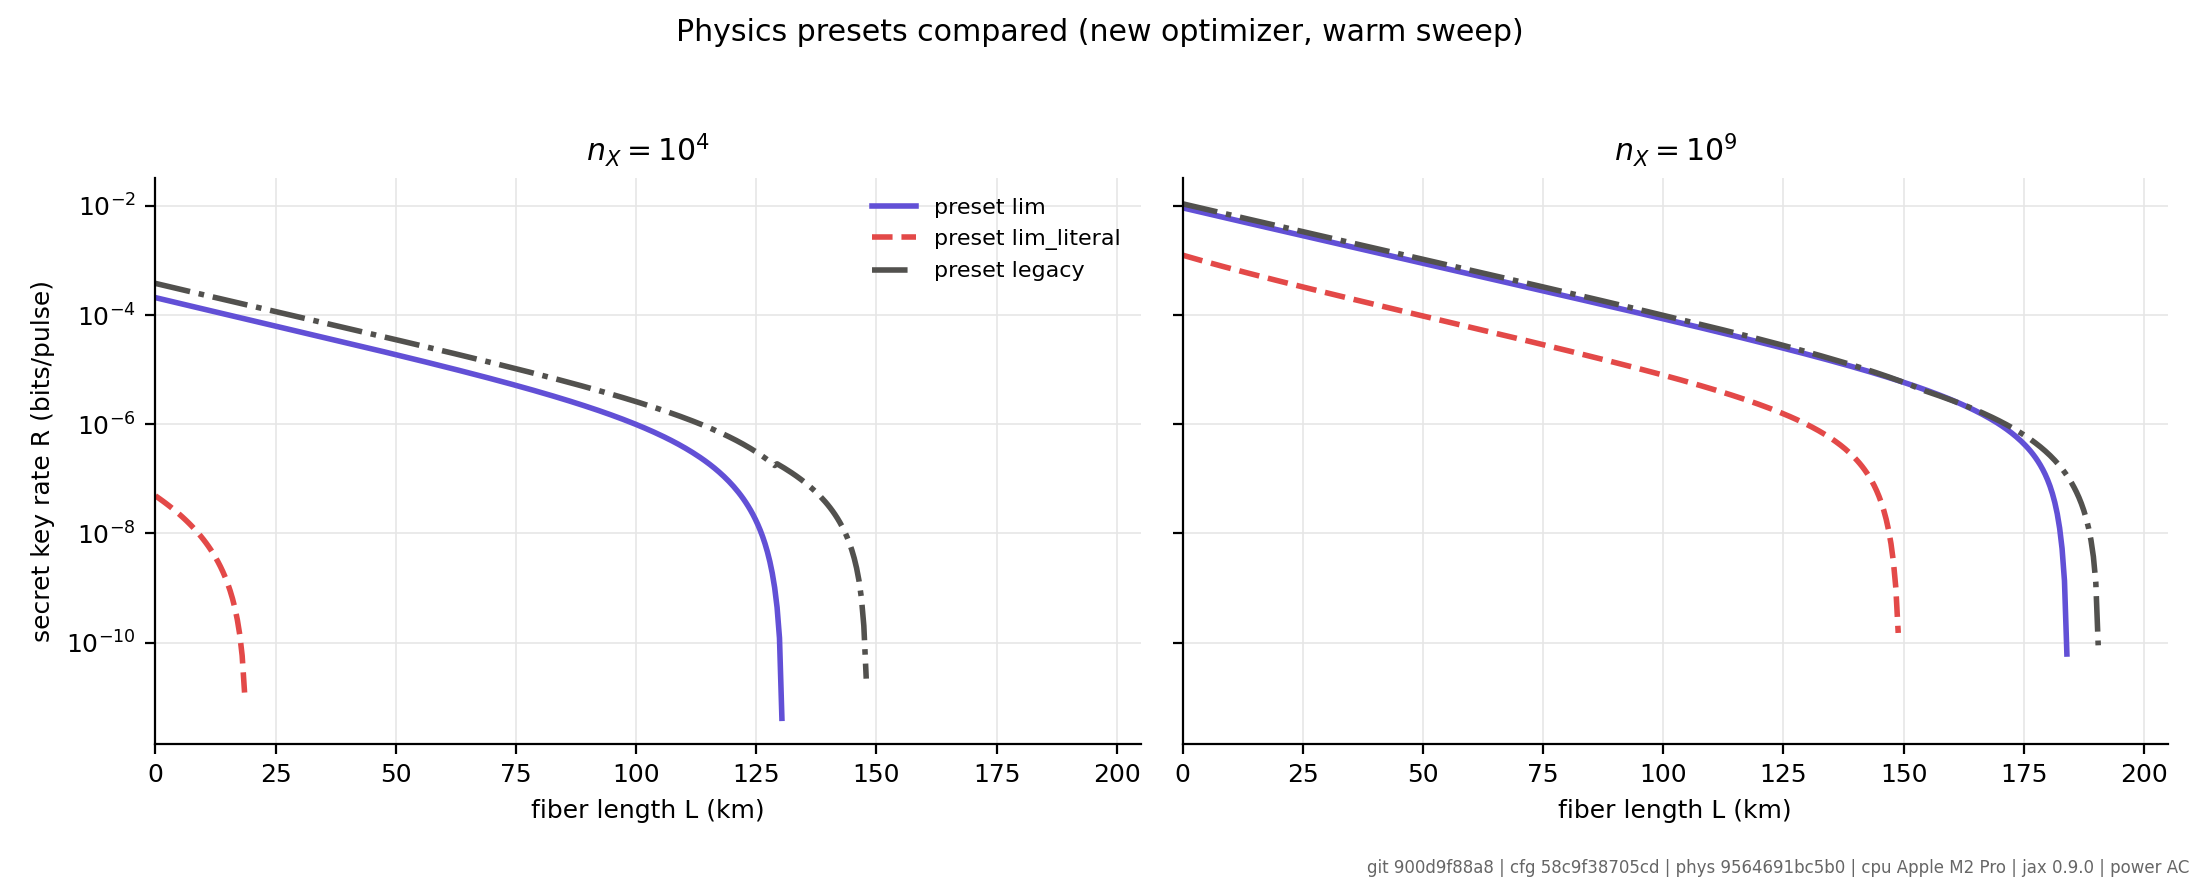
\includegraphics[width=0.85\linewidth]{fig2_presets.png}
\caption{$R(L)$ under the three presets for $n_X=10^4$ and $10^9$ (\texttt{fig2}).}
\end{figure}
\begin{figure}[H]\centering
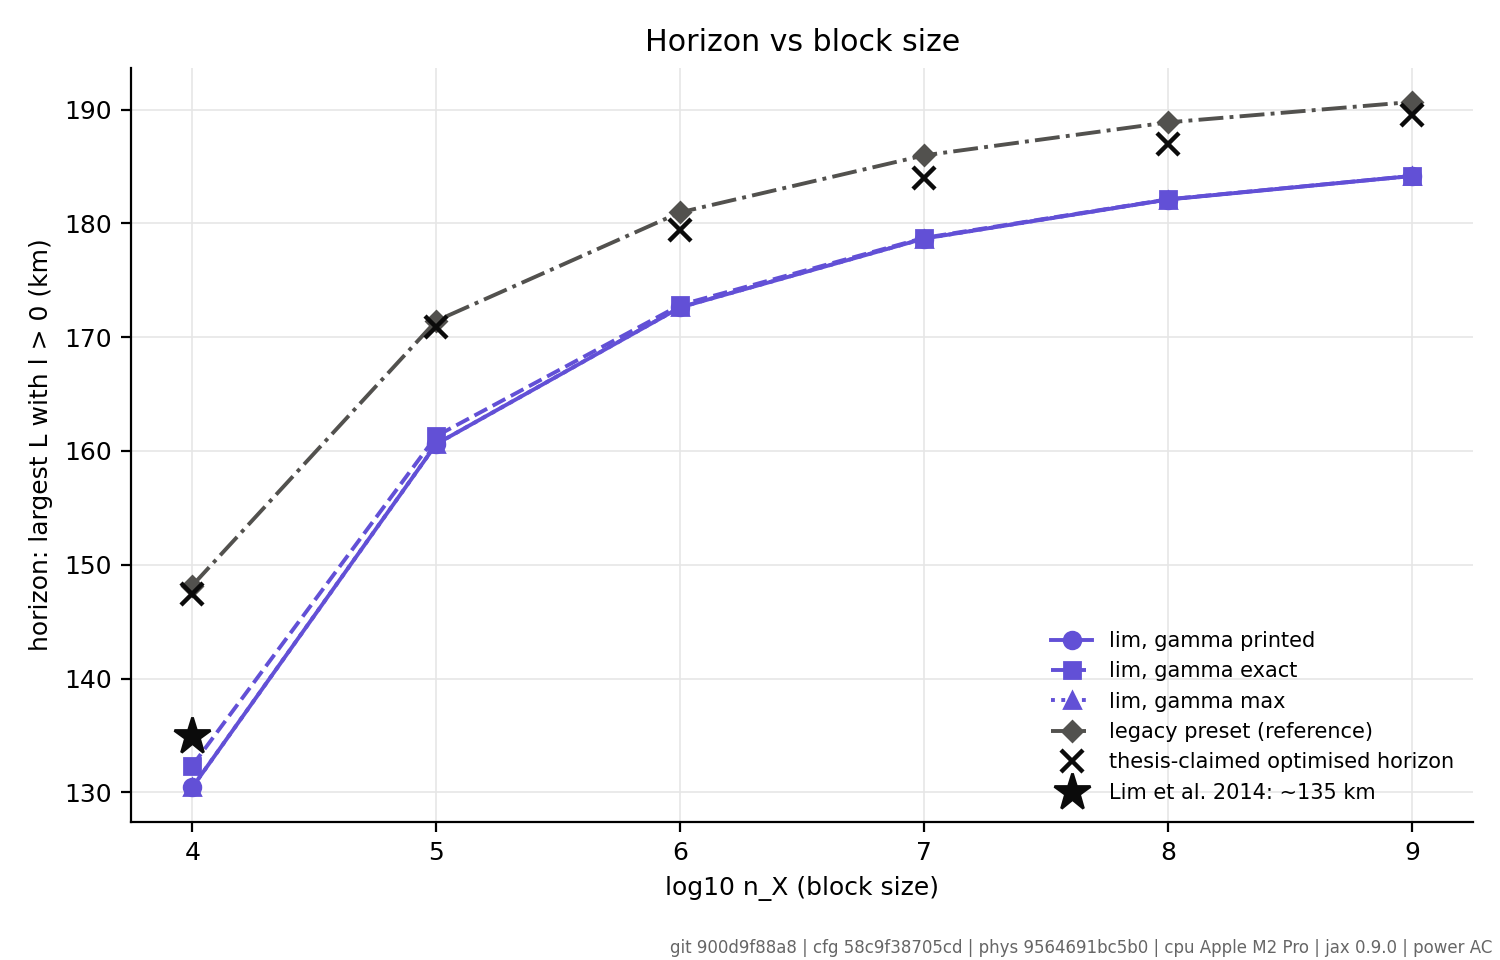
\includegraphics[width=0.8\linewidth]{fig3_horizon.png}
\caption{Horizon vs $n_X$: \plim\ with the printed, exact and max $\gamma$; \legacy; the horizons claimed in the
earlier thesis material; the paper's $\sim$135\,km (\texttt{fig3}).}
\end{figure}
\begin{figure}[H]\centering
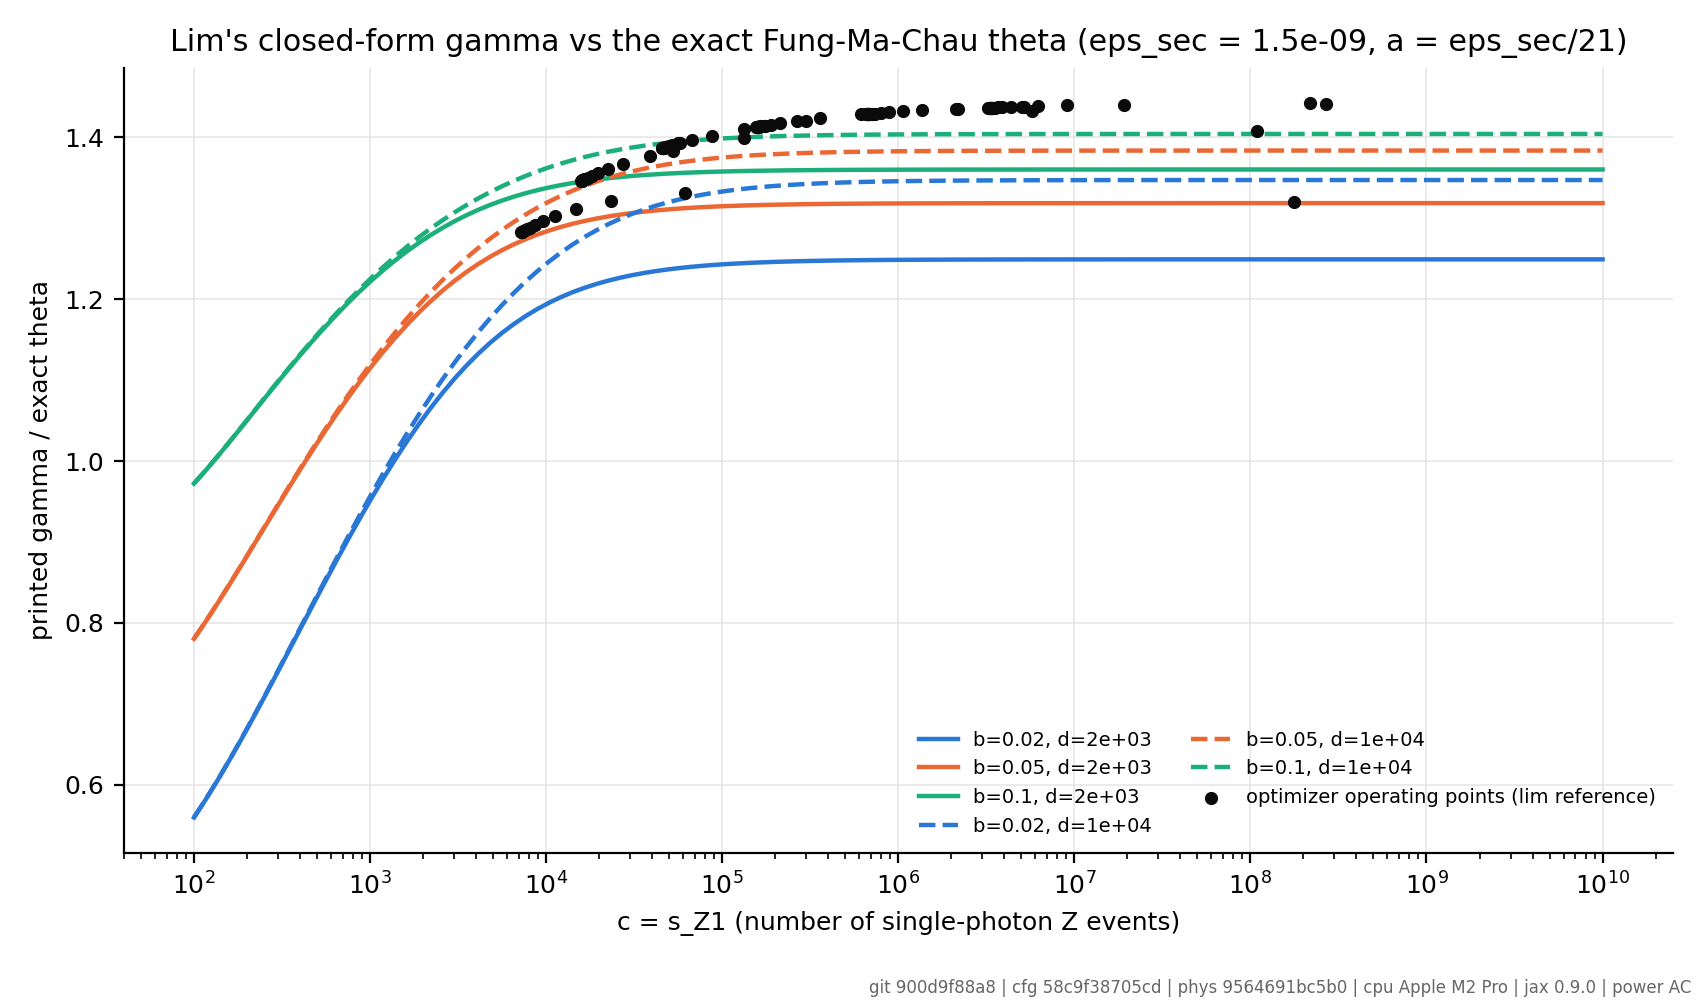
\includegraphics[width=0.8\linewidth]{fig9_gamma.png}
\caption{Ratio of the closed-form $\gamma$ to the exact Fung--Ma--Chau deviation; black points are the operating
points (\texttt{fig9}).}\label{fig:gamma}
\end{figure}

\section{Reproducibility}
\sloppy
\begin{itemize}
\item \texttt{python Optimization/run\_all.py} rebuilds the references, cross-checks, benchmarks, timings and
  analyses. Each step is recorded in \path{results/MANIFEST.json} with git commit, config hash, physics hash,
  hardware and power state.
\item \path{Optimization/report/make_numbers.py} writes \path{generated_numbers.tex}, which defines every
  \verb|\QKD...| value used here.
\item \path{Optimization/report/make_figures.py} writes the figures (git \texttt{900d9f88a8}, config
  \texttt{58c9f38705cd}).
\item Numbers marked \typed\ are copied from the result file named beside them.
\item The test suite passes: 34 tests, \texttt{python -m unittest discover tests}.
\item The run log with every measured value is in \texttt{STATUS.md}.
\end{itemize}

\section*{References}
\begin{enumerate}\small
\item C.~C.~W.~Lim, M.~Curty, N.~Walenta, F.~Xu, H.~Zbinden, \emph{Concise security bounds for practical
  decoy-state quantum key distribution}, Phys.\ Rev.\ A \textbf{89}, 022307 (2014), arXiv:1311.7129.
\item C.-H.~F.~Fung, X.~Ma, H.~F.~Chau, \emph{Practical issues in quantum-key-distribution postprocessing},
  Phys.\ Rev.\ A \textbf{81}, 012318 (2010), arXiv:0910.0312.
\end{enumerate}

\end{document}
